\documentclass{beamer}
\usetheme{Warsaw}


\iftrue

\setbeamercolor{normal text}{fg=white,bg=black!90}
\setbeamercolor{structure}{fg=white}

\setbeamercolor{alerted text}{fg=red!85!black}

\setbeamercolor{item projected}{use=item,fg=black,bg=item.fg!35}

\setbeamercolor*{palette primary}{use=structure,fg=structure.fg}
\setbeamercolor*{palette secondary}{use=structure,fg=structure.fg!95!black}
\setbeamercolor*{palette tertiary}{use=structure,fg=structure.fg!90!black}
\setbeamercolor*{palette quaternary}{use=structure,fg=structure.fg!95!black,bg=black!80}

\setbeamercolor*{framesubtitle}{fg=white}

\setbeamercolor*{block title}{parent=structure,bg=black!60}
\setbeamercolor*{block body}{fg=black,bg=black!10}
\setbeamercolor*{block title alerted}{parent=alerted text,bg=black!15}
\setbeamercolor*{block title example}{parent=example text,bg=black!15}

\fi


\begin{document}

{
    \usebackgroundtemplate
    {
        \vbox to \paperheight{\vfil\hbox to \paperwidth{\hfil

        {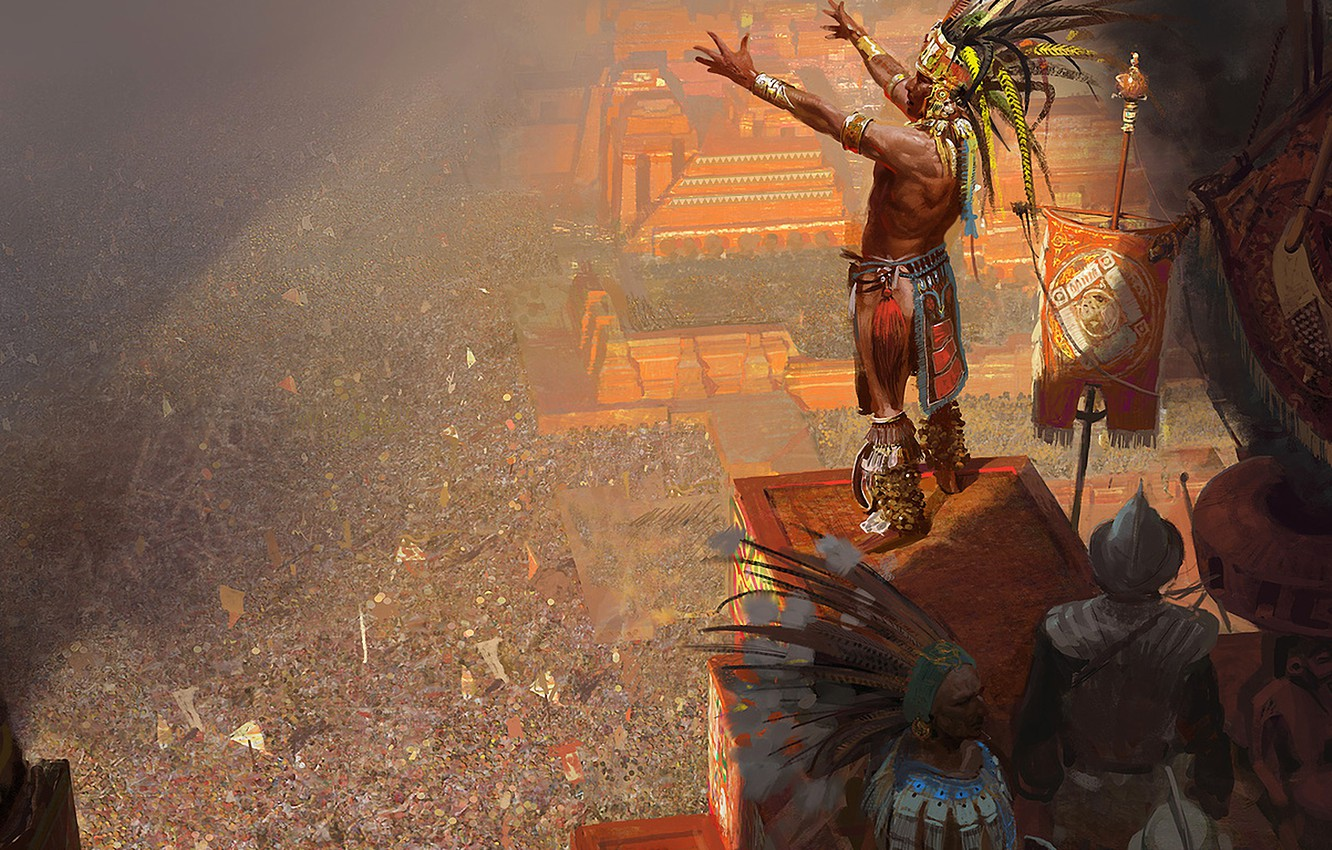
\includegraphics[width=5.05in]{../images/aztec.jpg}}

        \hfil}\vfil}
    }

    \begin{frame}
     \centering
     {
        \begin{minipage}{10cm}
           {\LARGE \color{white}{\bf algorithms for robotics}} \\
           {\LARGE \color{white}{\bf Michal CHOVANEC, PhD.}} \\
       \end{minipage}
     }

    \end{frame}
}


\begin{frame}
  
  \frametitle{\bf overview}

  \begin{itemize}
    \item noise reduction             : digital filters, Kalman filter
    \item control                     : PID, LQR, MPC
    \item motor controll              : park, clark transformations, real time PID
    \item planning, decision making   : image segmentation, reinforcement learning
  \end{itemize}
    
\end{frame}


\begin{frame}
  
  \frametitle{\bf digital filters}

  \begin{itemize}

    \item low pass filter (1st order)
      \begin{align*}
        y_{n}&= (1 - a)y_{n-1} + a x_{n} \\
        a &= \frac{\Delta t}{RC + \Delta t}
      \end{align*}
  

    \item resonant filter (2nd order)
      \begin{align*}
        y_{n}&= a_{1}y_{n-1} + a_{2}y_{n-2} + b_{0}x_{n} + b_{1}x_{n-1} + b_{2}x_{n-2} 
      \end{align*}

  \end{itemize}

  
\end{frame}


\begin{frame}
  
  \frametitle{\bf digital filters - usage}

    \centering{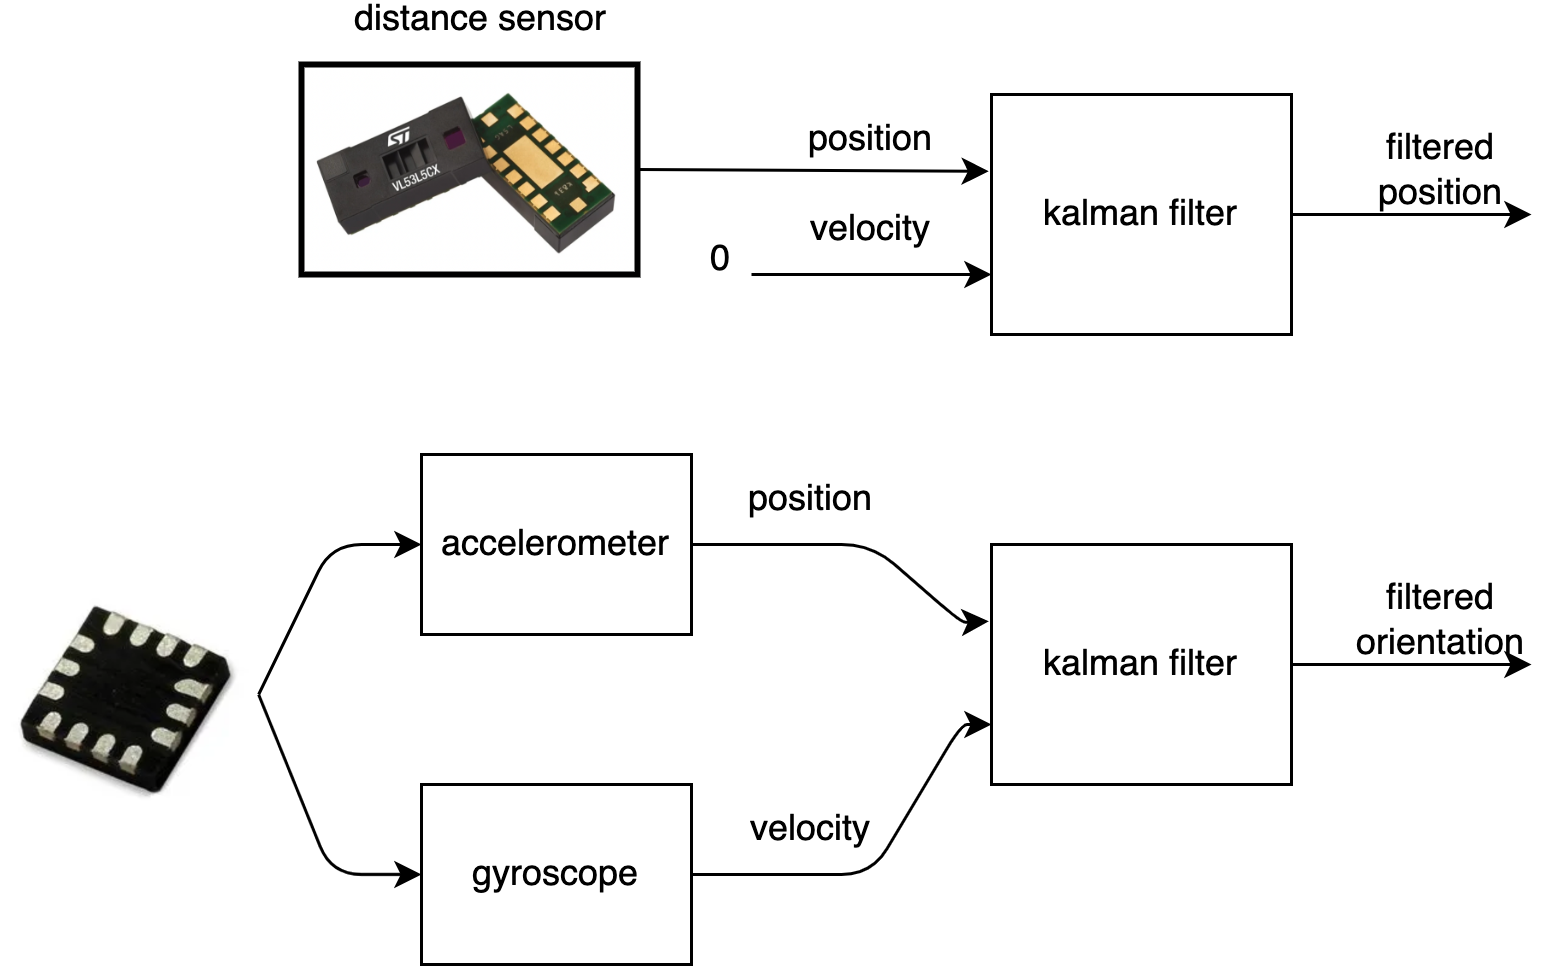
\includegraphics[scale=0.8]{../diagrams/filters/filters.png}}

\end{frame}

\begin{frame}
  
  \frametitle{\bf digital filters - low pass vs Kalman}

    \centering{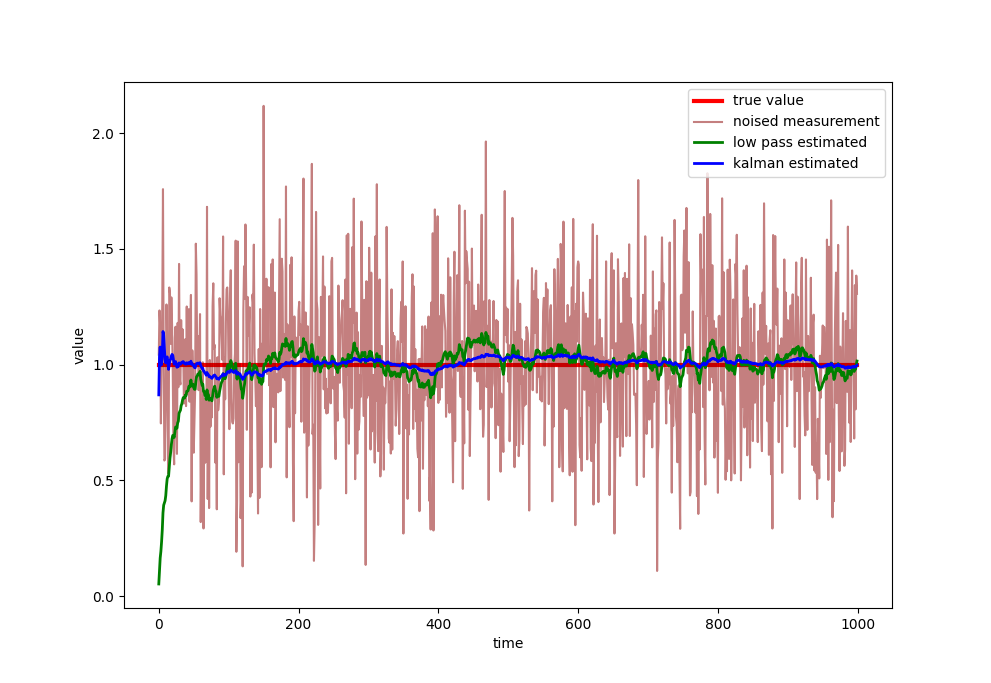
\includegraphics[scale=0.25]{../images/kalman_constant.png}}
    \centering{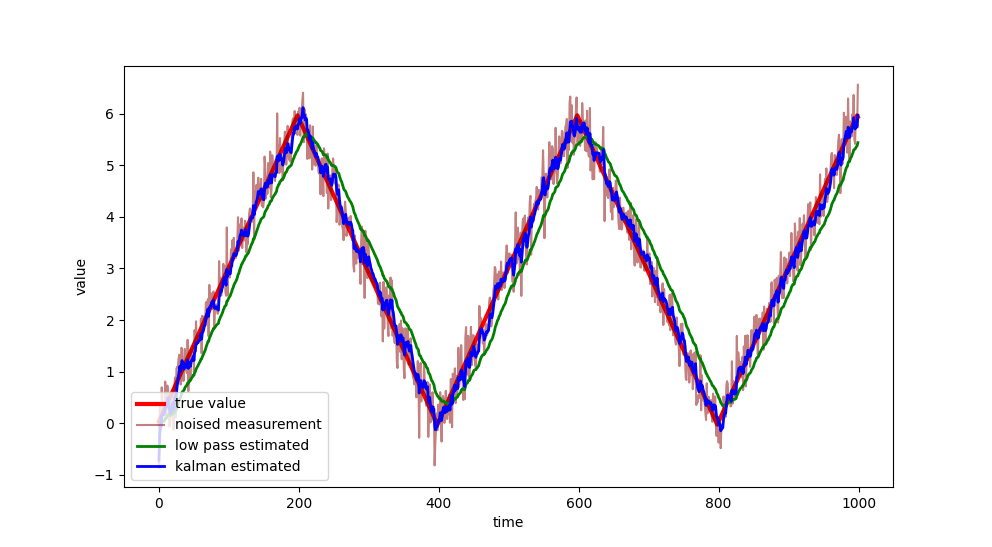
\includegraphics[scale=0.25]{../images/kalman_tracking.png}}

\end{frame}


\begin{frame}
  
  \frametitle{\bf 1D kalman is simple}    

    \begin{columns}

      \begin{column}{0.5\textwidth}
        \centering{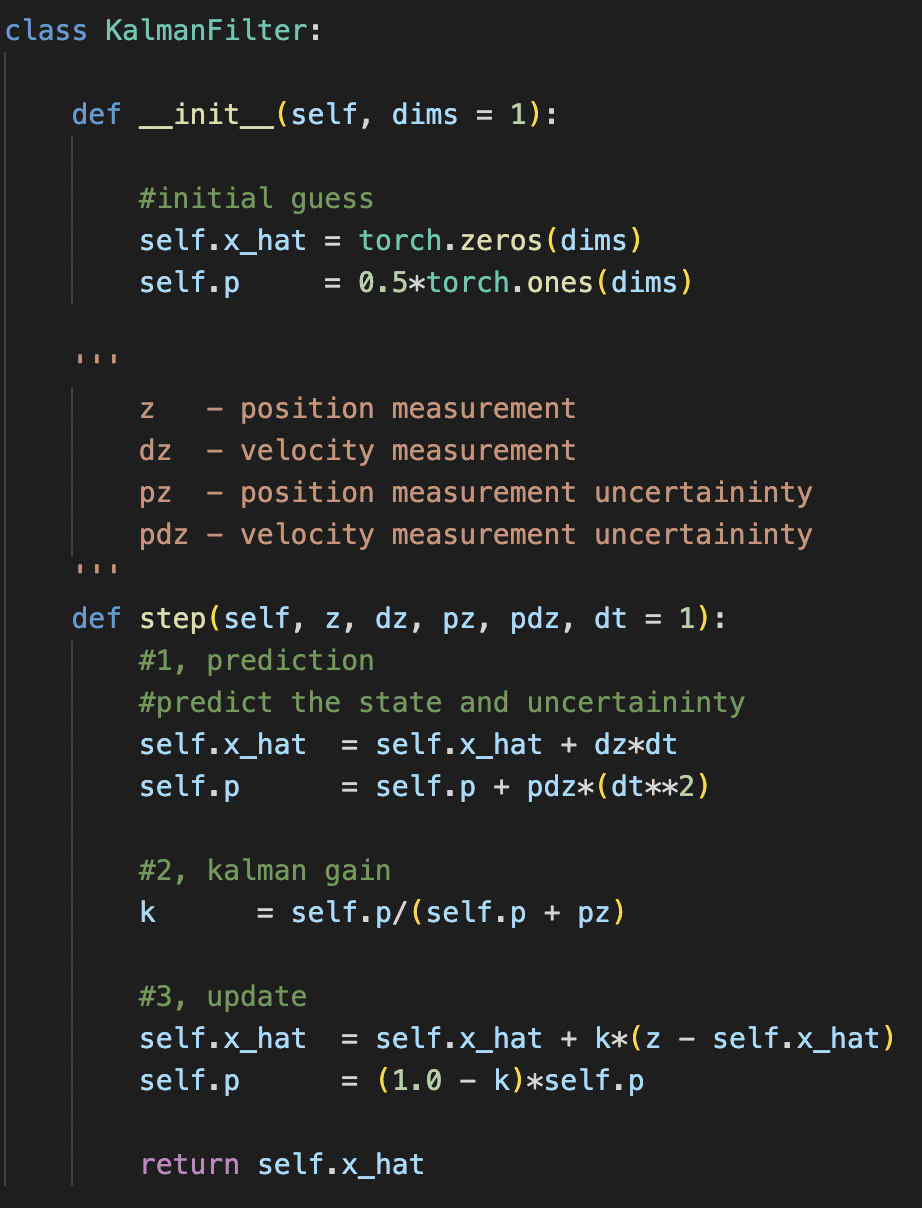
\includegraphics[scale=0.25]{../images/kalman_1d.png}}
      \end{column}
  
      \begin{column}{0.5\textwidth}
        \begin{itemize}
          \item 1, calibrate sensor variance (pz, pdz)
          \item 2, measure position z \\ and velocity v
          \item 3, dynamics model $$z_{n-1} = z_{n} + v_{n}dt$$
          \item 4, compute filter step
        \end{itemize}
      \end{column}
  
    \end{columns}

\end{frame}



\begin{frame}
  
  \frametitle{\bf usage}    

    \begin{columns}

      \begin{column}{0.5\textwidth}
        \centering{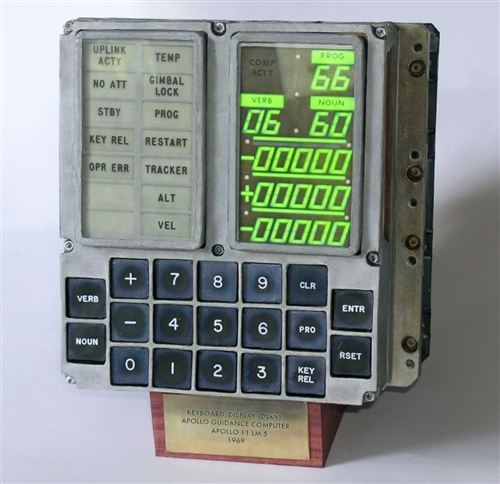
\includegraphics[scale=0.25]{../images/dsky.jpeg}}
        \centering{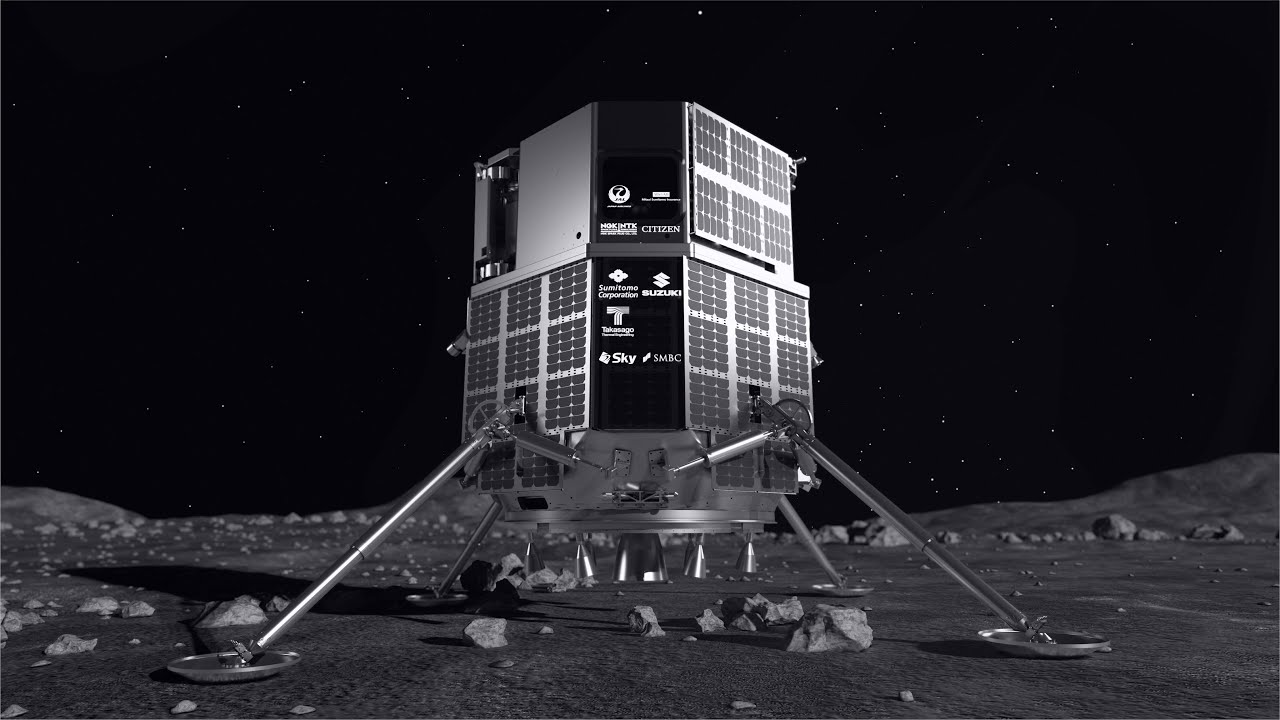
\includegraphics[scale=0.09]{../images/hakuto.jpg}}
      \end{column}
  
      \begin{column}{0.5\textwidth}
        \begin{itemize}
          \item sensors de-noising 
          \item sensors fusion \\ (gyro + accelerometer), GPS
          \item navigation, error checking
          \item Apollo guidance computer (Apollo 8, 1968)
          \item Hakuto lander crash !!! (2023, April 2023)
        \end{itemize}
      \end{column}
  
    \end{columns}

\end{frame}



\begin{frame}
  
  \frametitle{\bf controll : PID vs LQR}    

    \centering{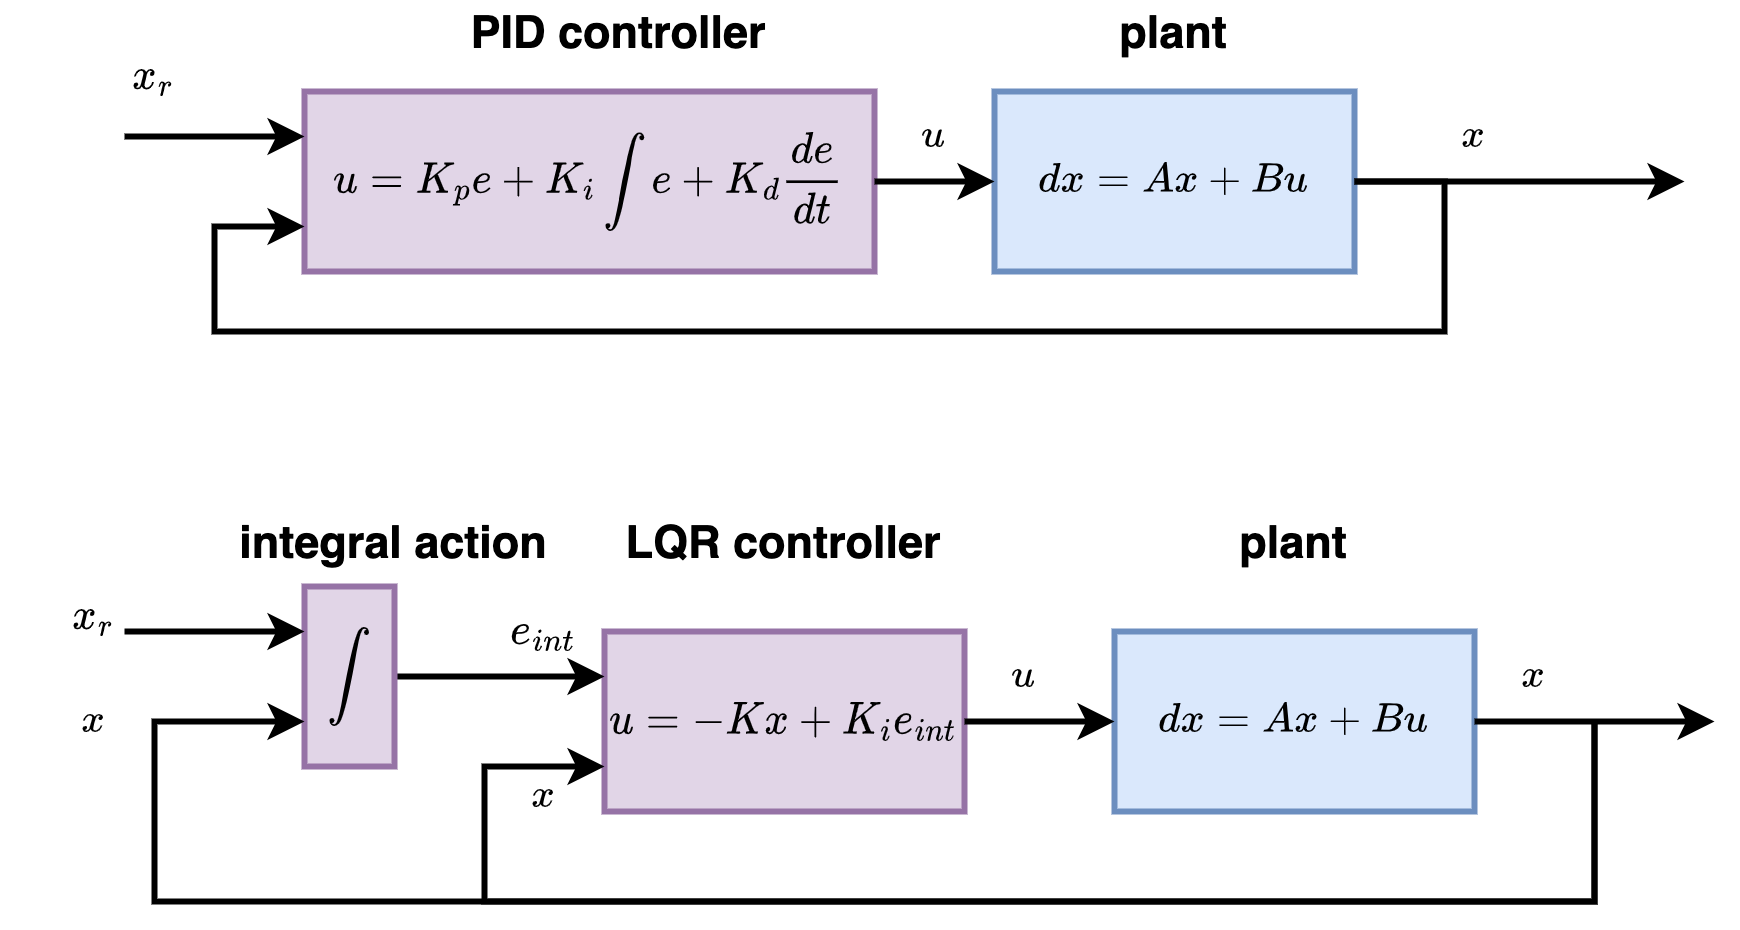
\includegraphics[scale=0.5]{../diagrams/controll/control-lqr_pid.png}}

    \begin{columns}

      \begin{column}{0.5\textwidth}
        \begin{itemize}
          \item PID
          \item single input, single output
          \item simple systems (motor control, temperature ...)
          \item empirical "tunning" 
        \end{itemize}
      \end{column}
  
      \begin{column}{0.5\textwidth}
        \begin{itemize}
          \item LQR
          \item multiple inputs, multiple outputs
          \item complex dynamics (drones, F16, rockets, walking robot, segway)
          \item exact solution
          \item robust
        \end{itemize}
      \end{column}
  
    \end{columns}


\end{frame}


\begin{frame}
  
  \frametitle{\bf servo state space model}    

    \centering{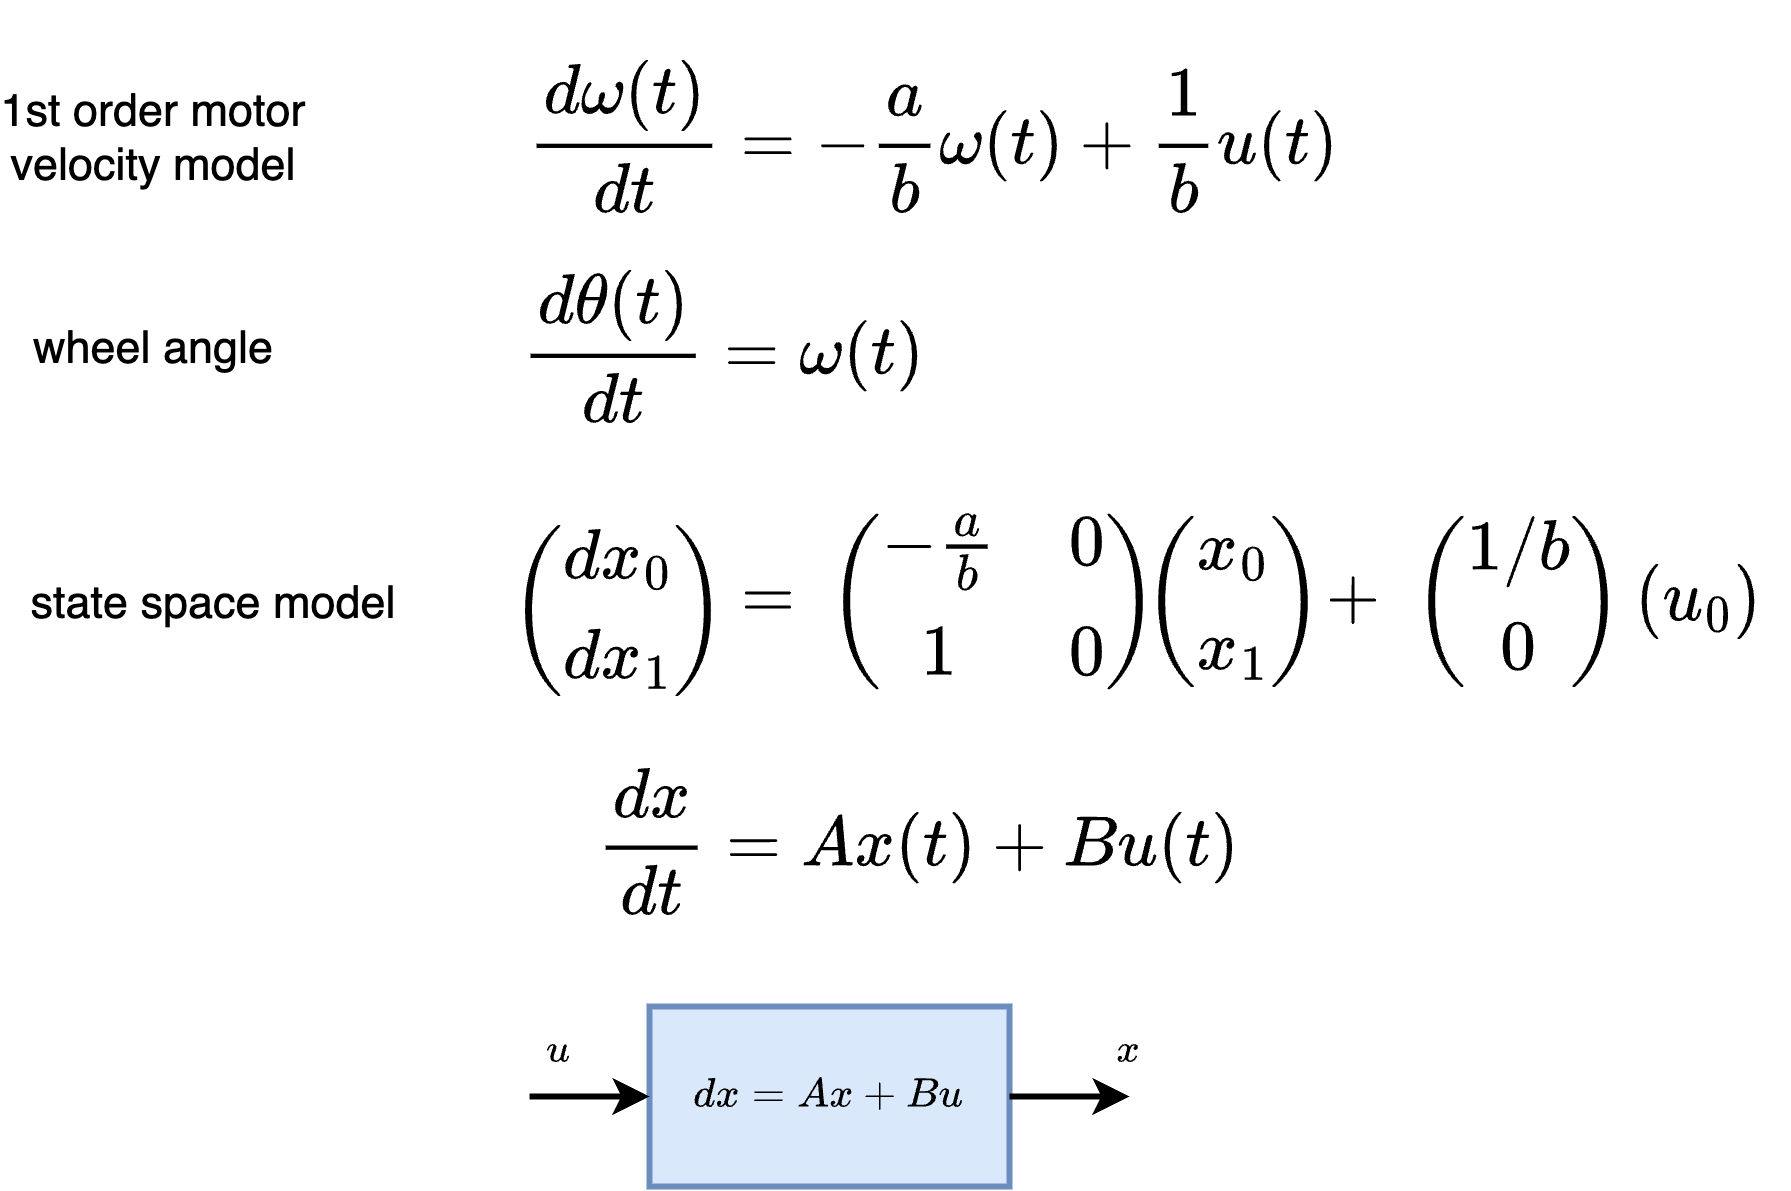
\includegraphics[scale=0.5]{../diagrams/controll/control-servo.png}}

\end{frame}

\begin{frame}
  
  \frametitle{\bf controller synthesis}    
  \centering{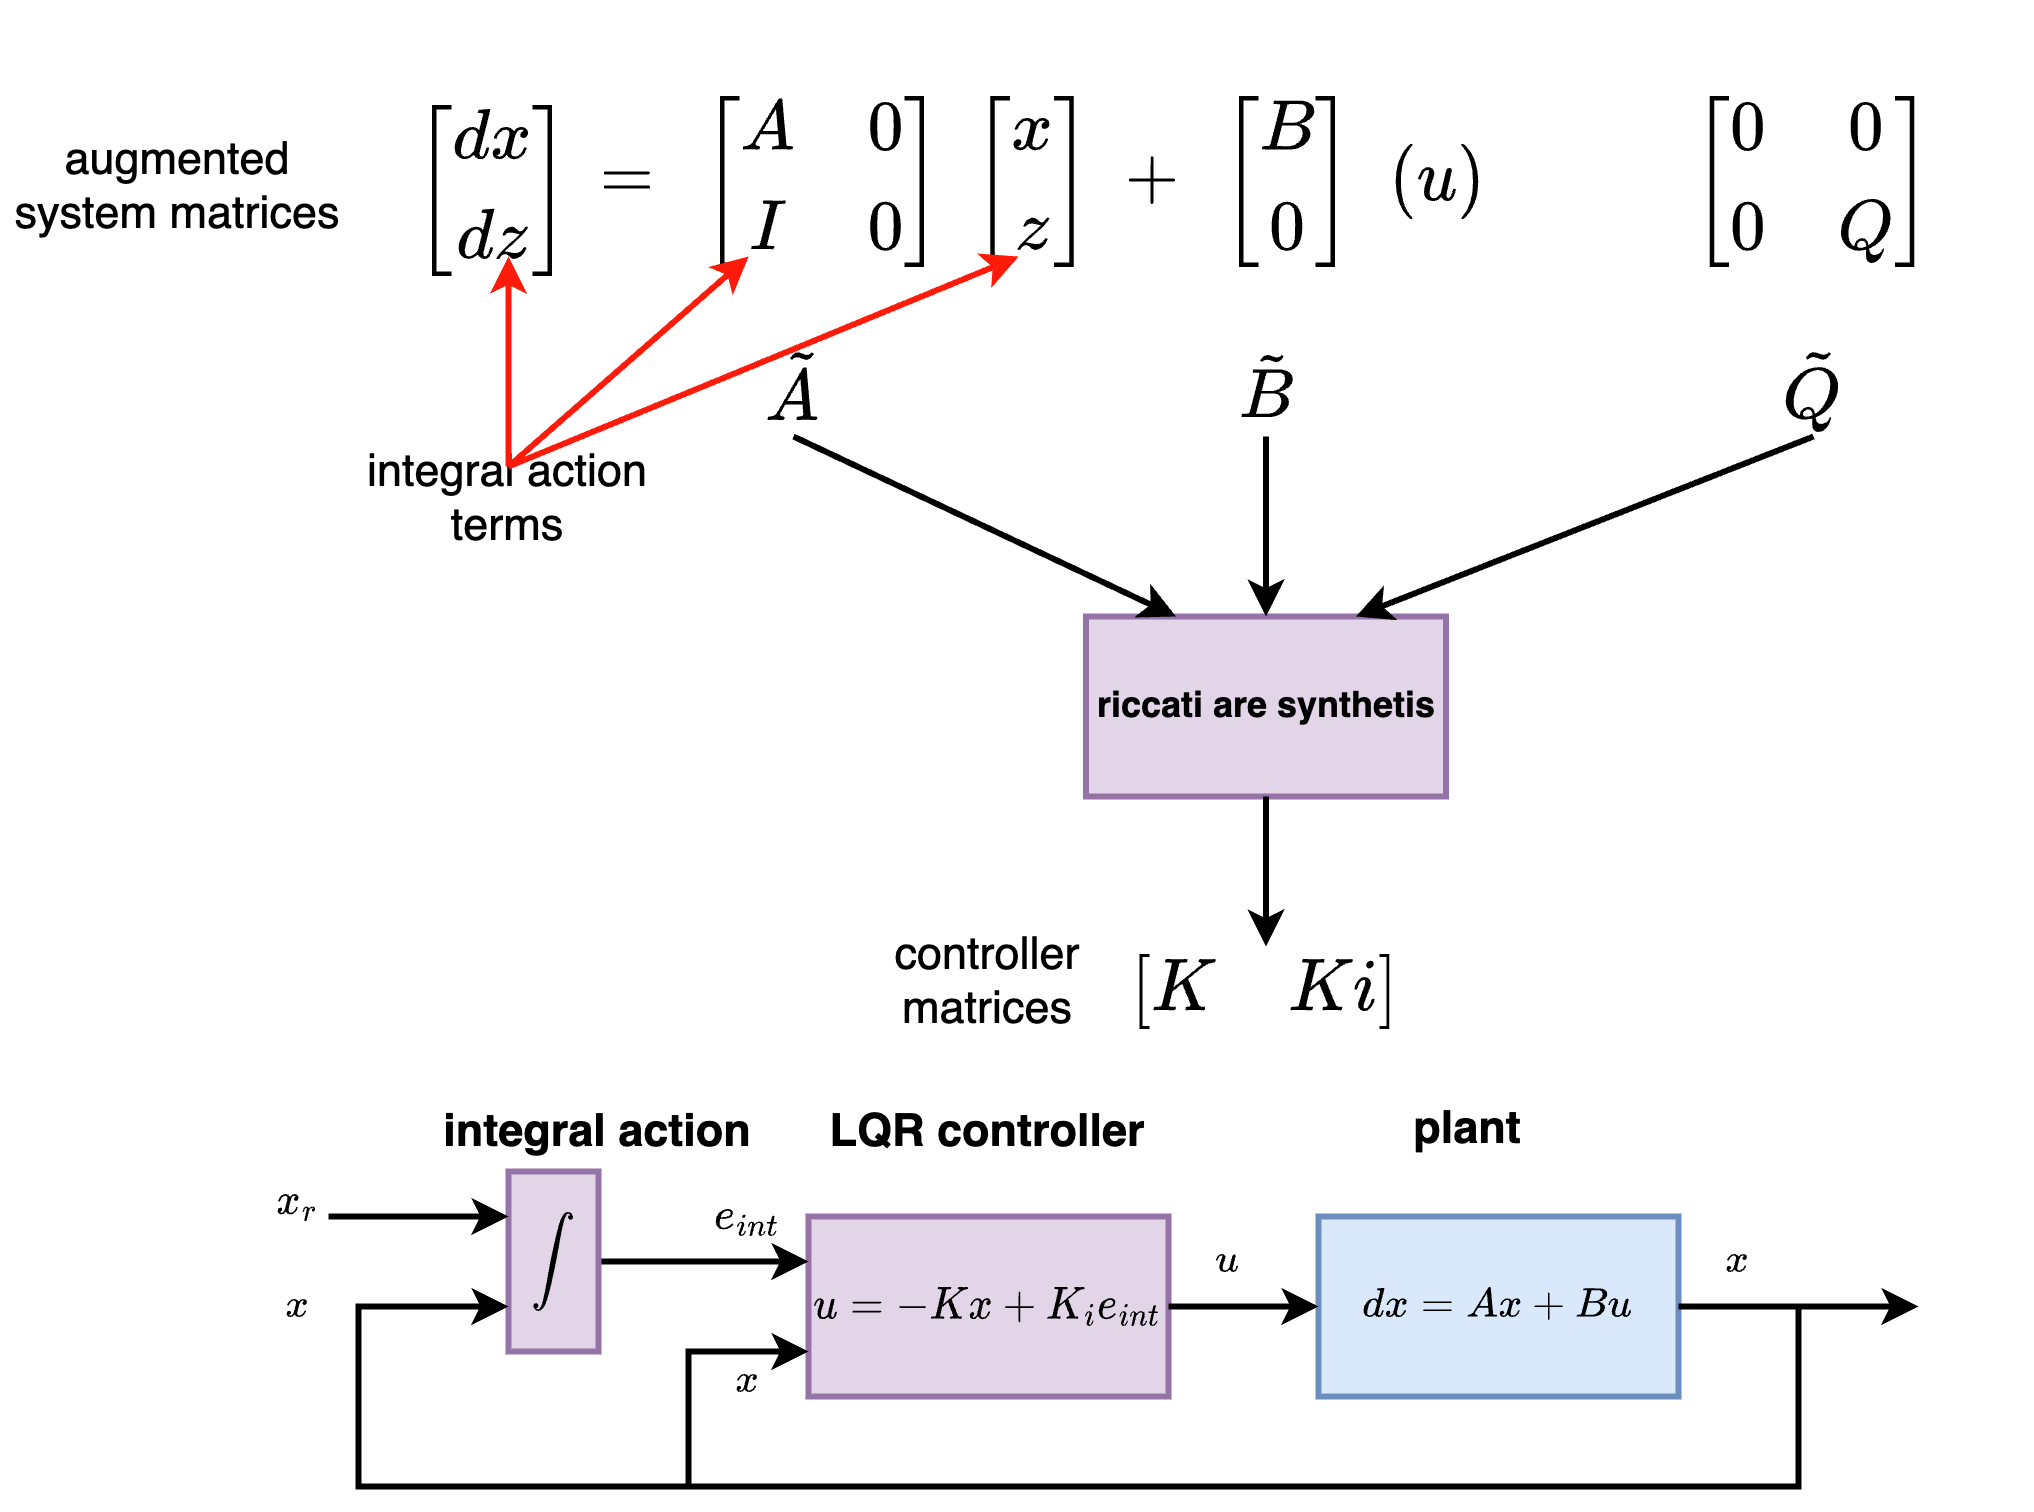
\includegraphics[scale=0.45]{../diagrams/controll/control-lqri_synth.png}}


\end{frame}

\begin{frame}
  
  \frametitle{\bf LQR for servo}    

    \centering{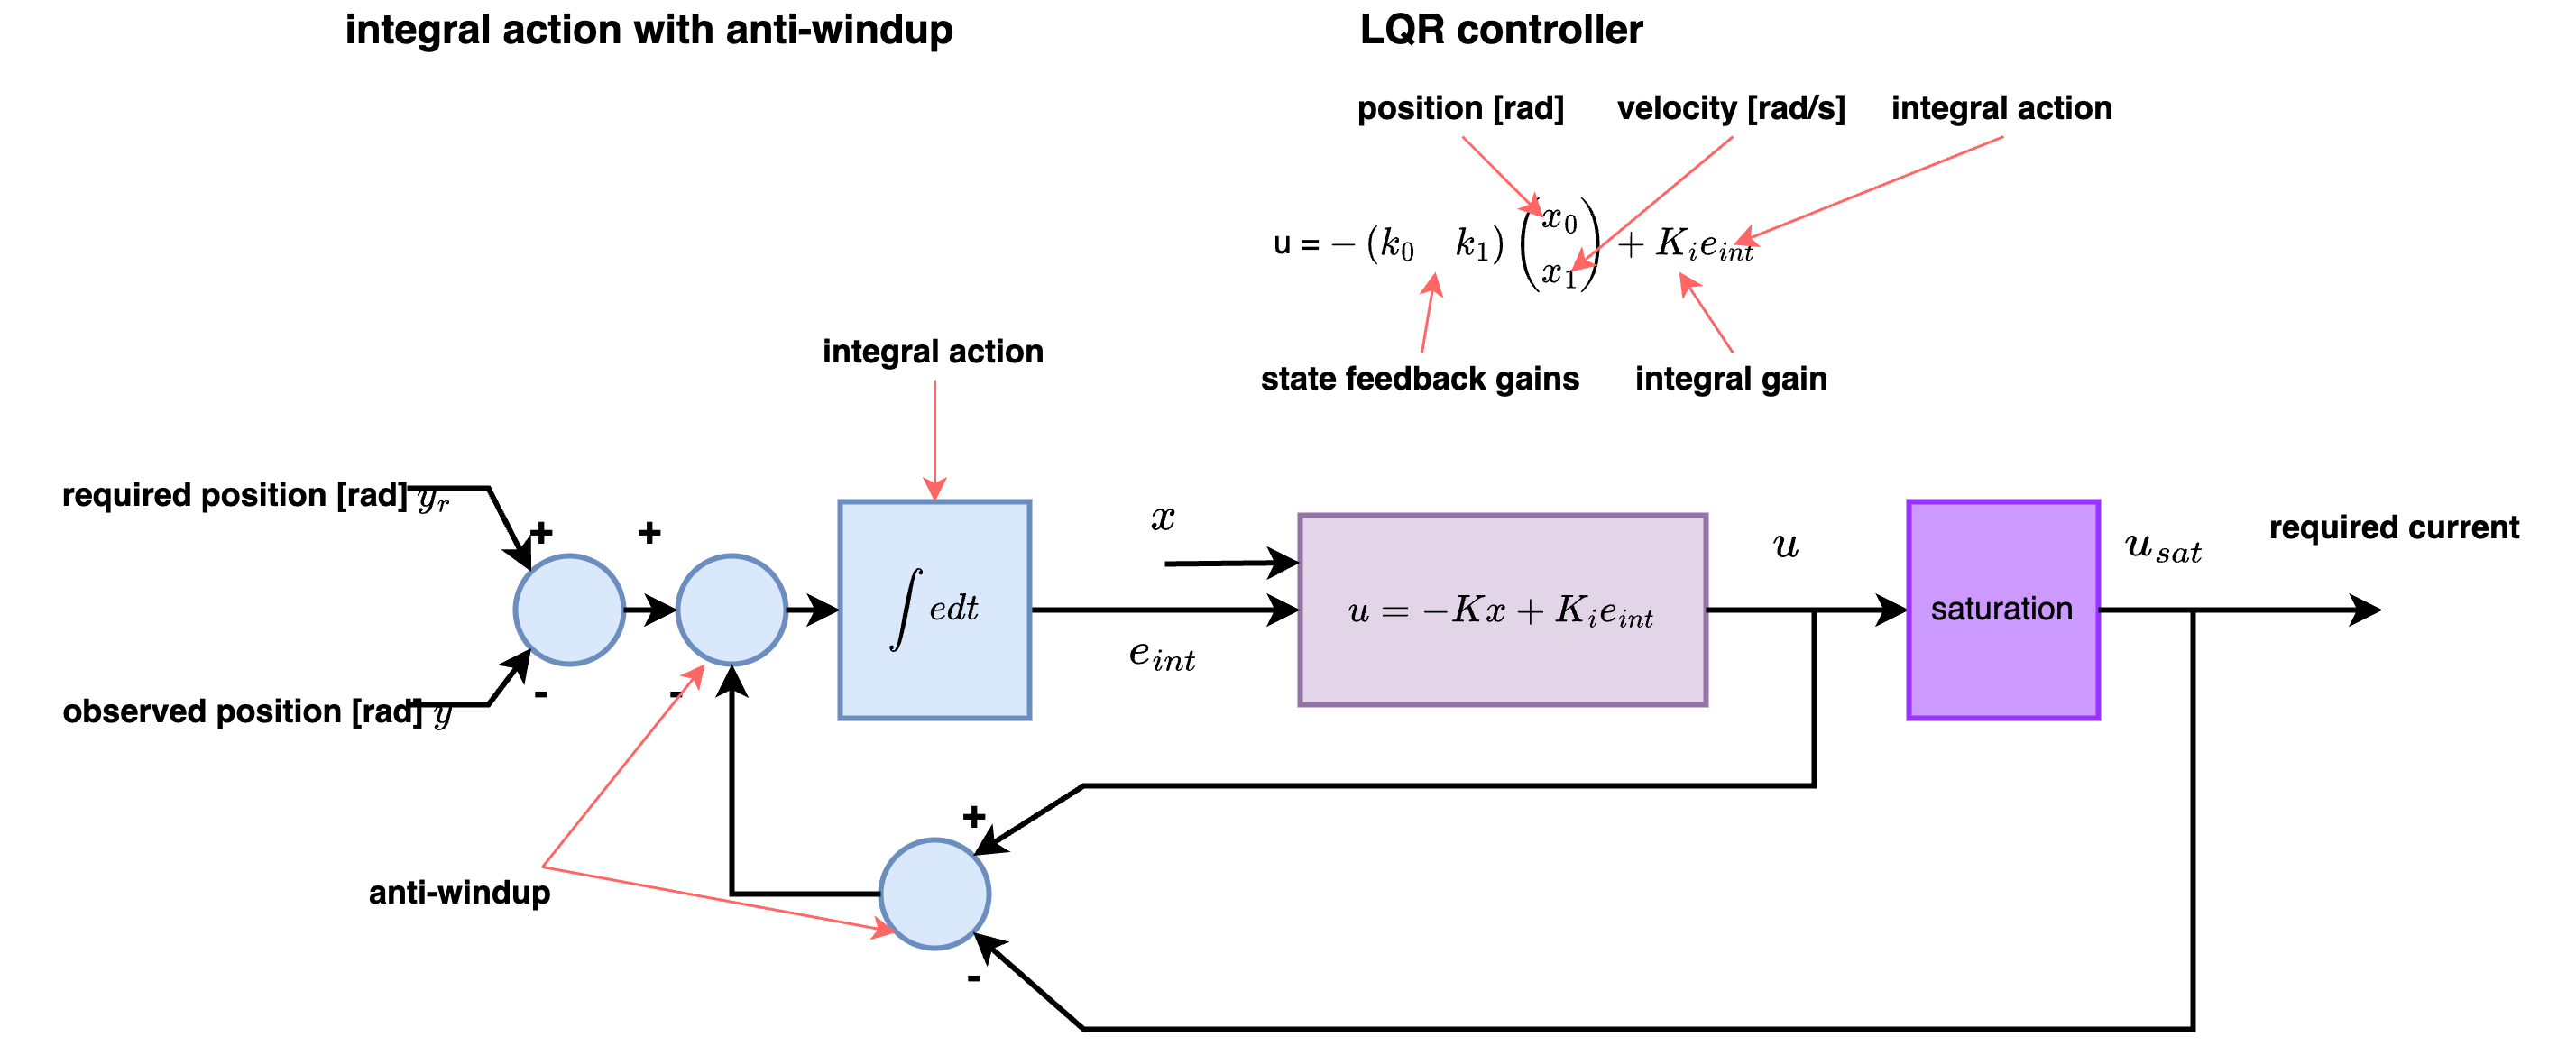
\includegraphics[scale=0.45]{../diagrams/controll/motor_control-lqr.png}}

\end{frame}





\begin{frame}
  
  \frametitle{\bf three phase motor controll}    

  \begin{columns}

    \begin{column}{0.5\textwidth}
      \centering{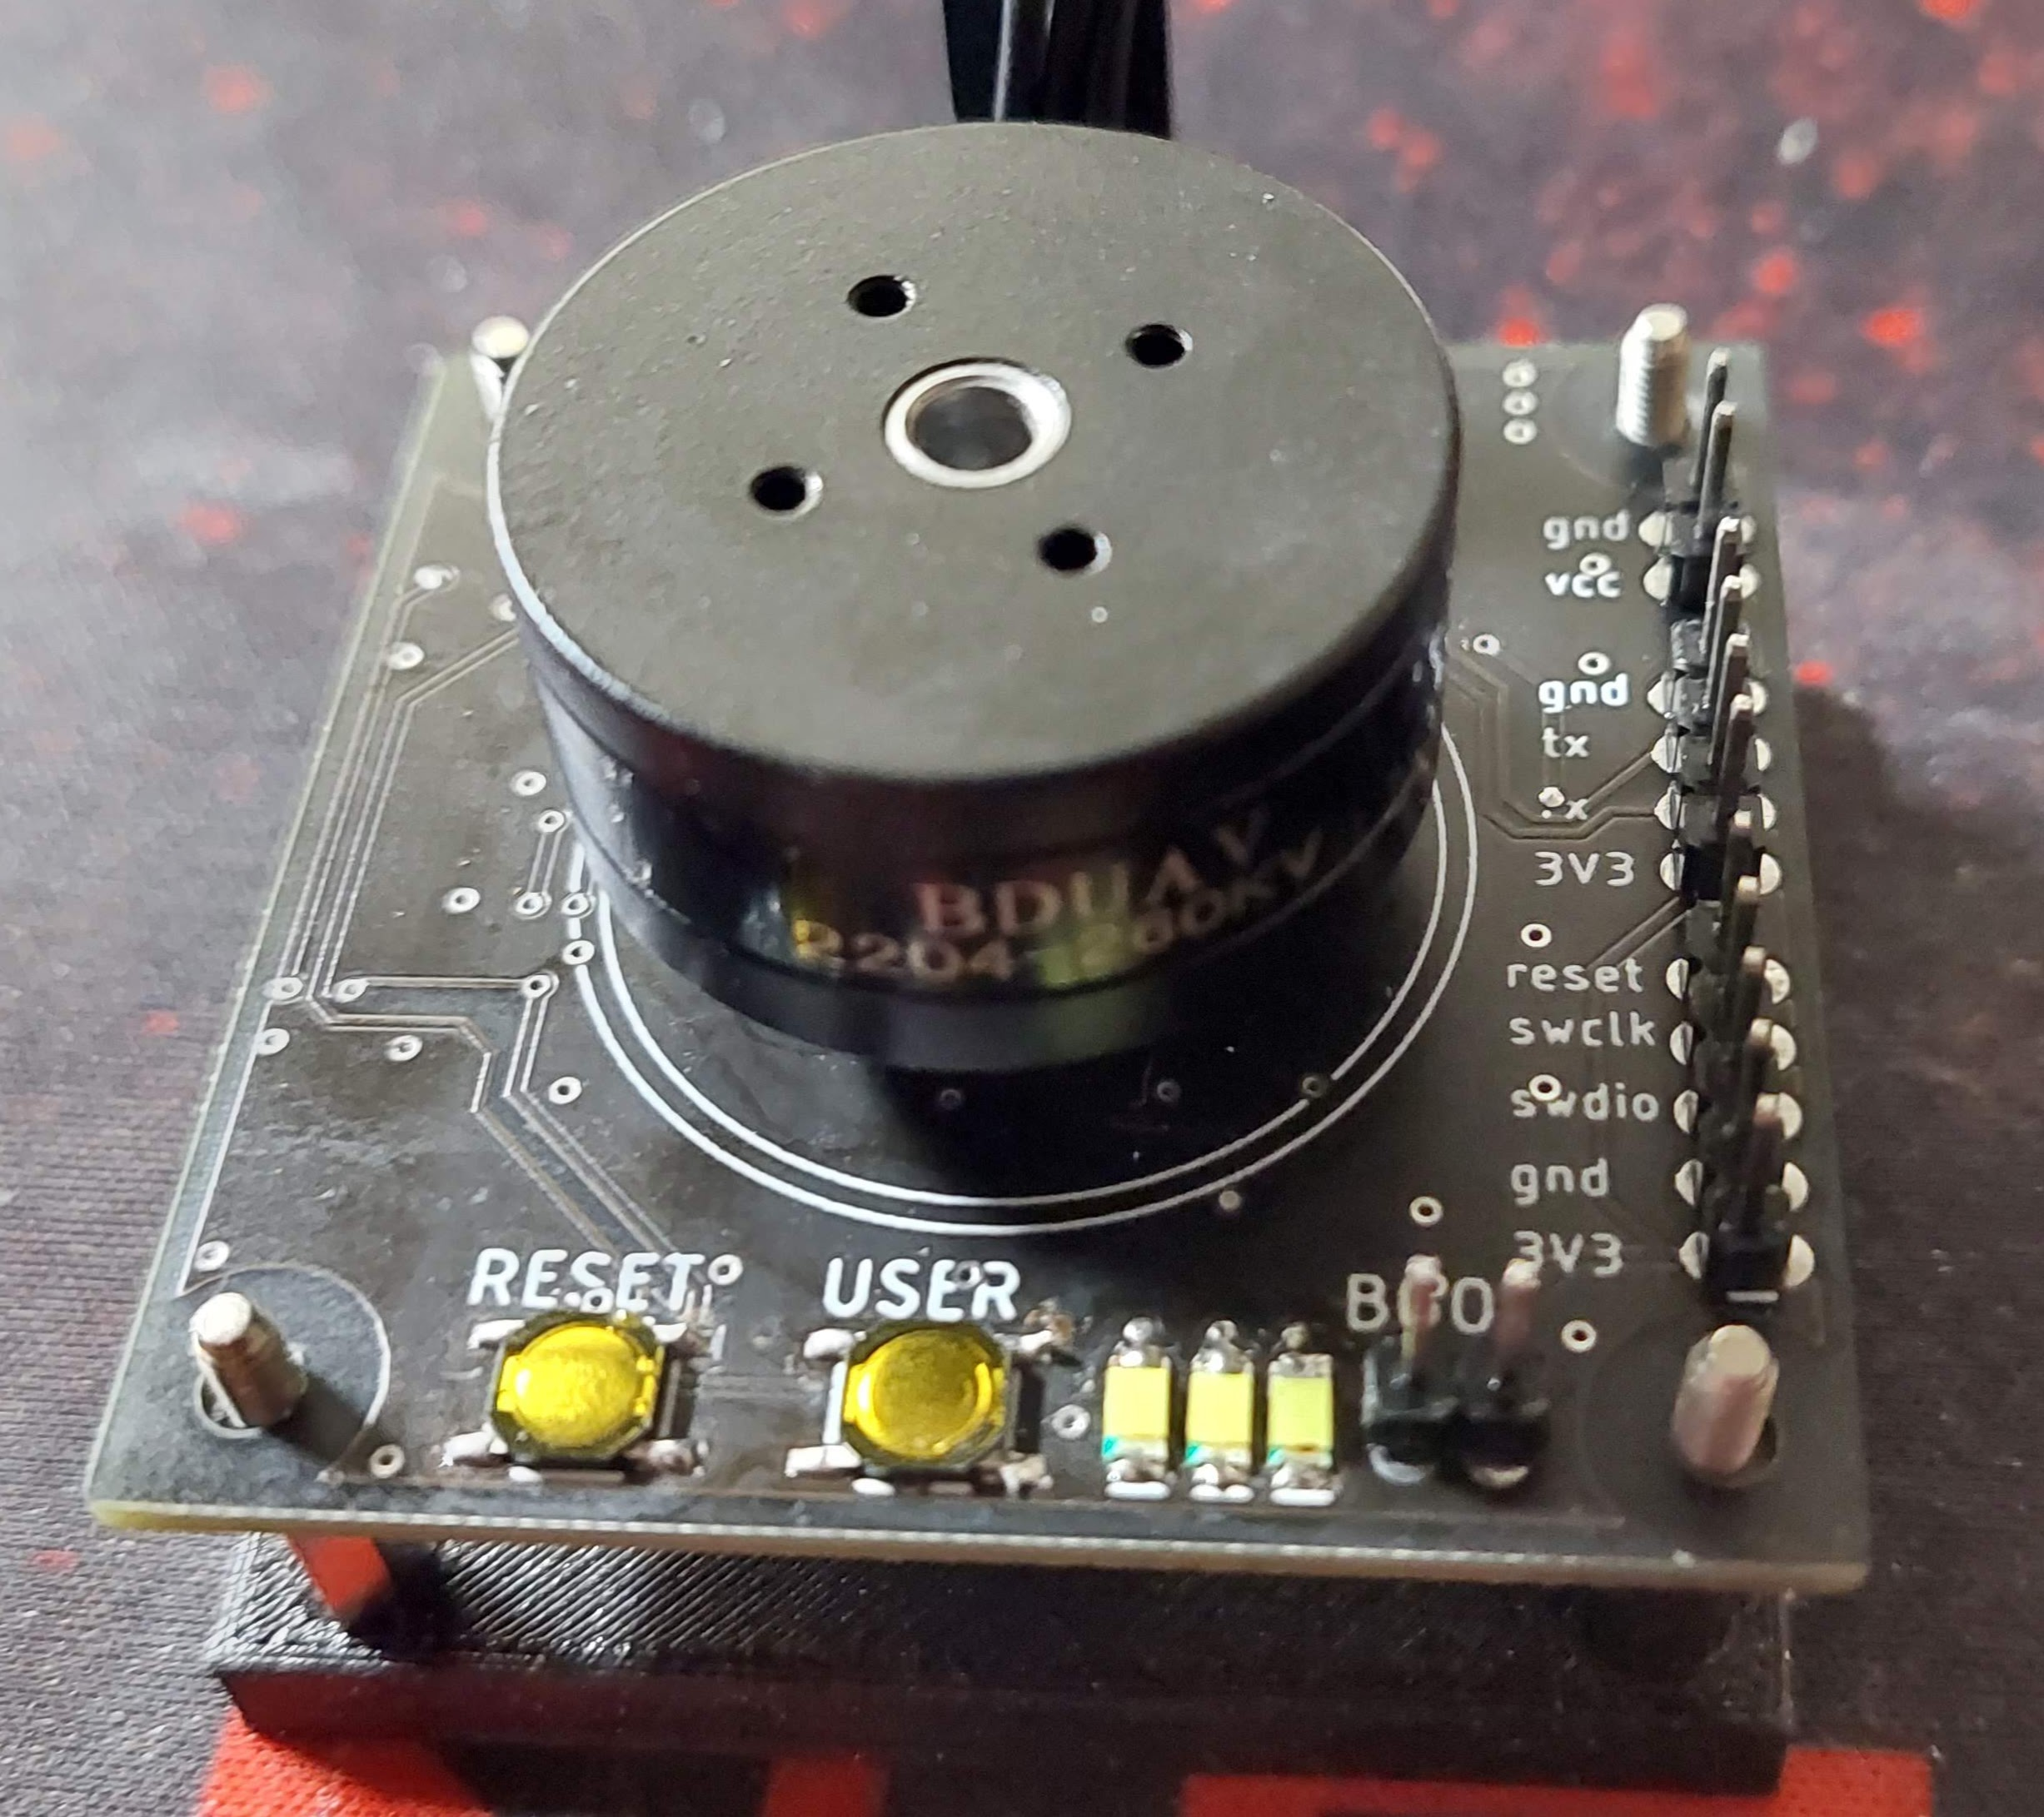
\includegraphics[scale=0.06]{../images/side_board.jpg}}
    \end{column}

    \begin{column}{0.5\textwidth}
      \begin{itemize}
        \item MCU     : stm32f051 \\ 
          - ARM cortex m0, 48MHz
        \item encoder : AS5600, 12bit
        \item driver  : MP6540H, 5A, 50V
      \end{itemize}
    \end{column}

  \end{columns}

\end{frame}



\begin{frame}
  
  \frametitle{\bf field oriented controll}    

  \centering{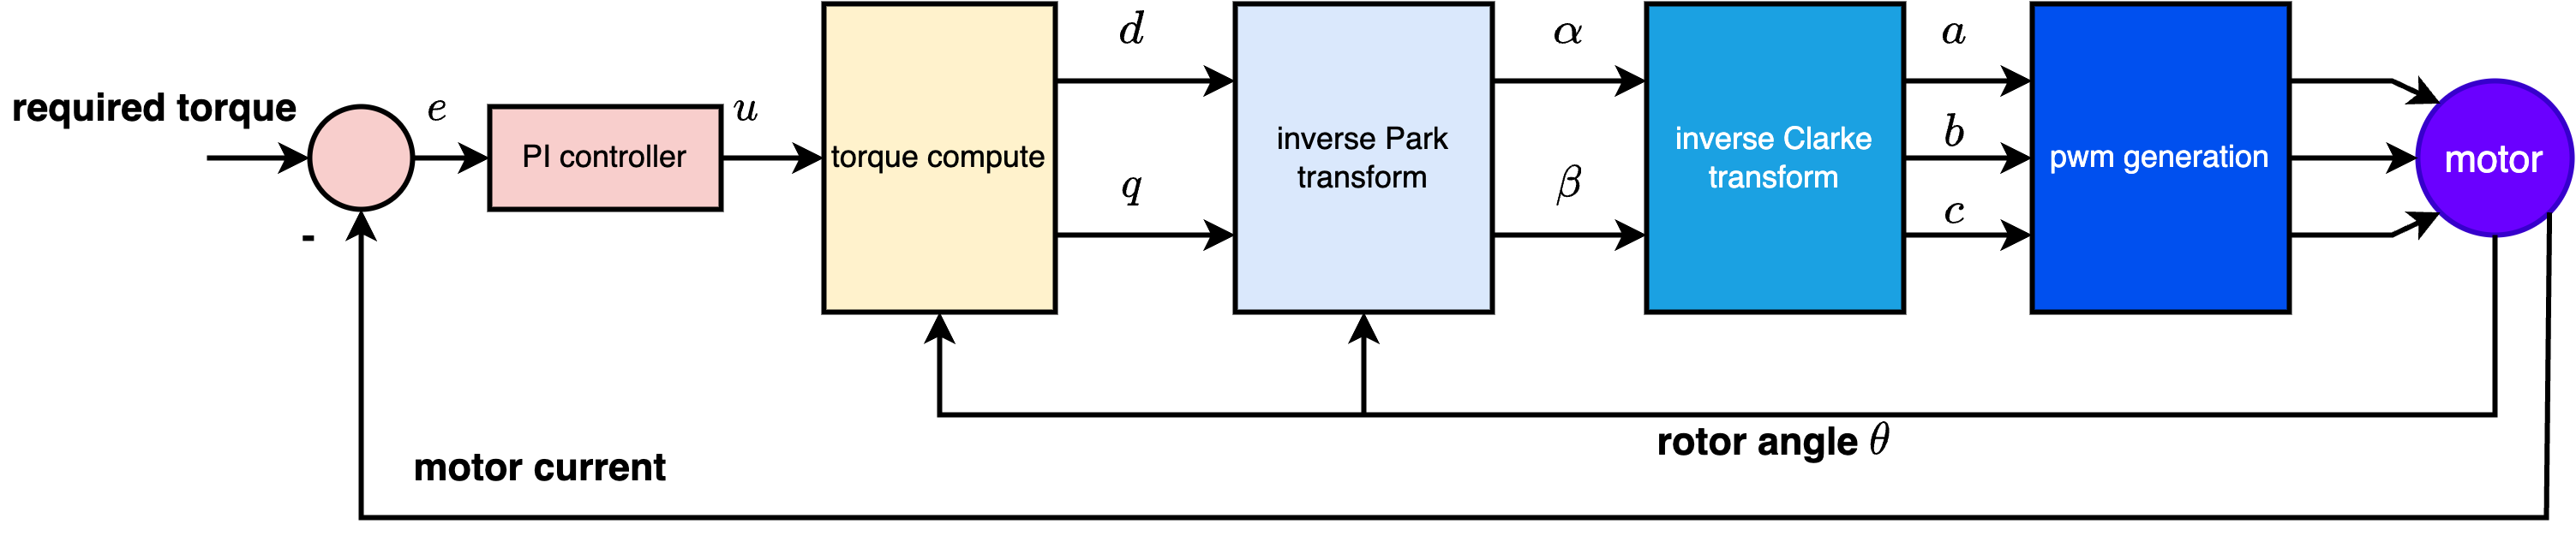
\includegraphics[scale=0.4]{../diagrams/controll/motor_control-inner_loop.png}}


  \begin{columns}

    \begin{column}{0.5\textwidth}
      trapezoidal control
      \begin{itemize}
        \item highest maximum speed
        \item lowest switching losses
        \item easiest implementation
      \end{itemize}
    \end{column}

    \begin{column}{0.5\textwidth}
      field oriented controll
      \begin{itemize}
        \item highest power output
        \item lowest noise
        \item best torque ripple
        \item maximum motor efficiency
        \item coding experience needed
      \end{itemize}
    \end{column}

  \end{columns}
  
\end{frame}


\begin{frame}
  
  \frametitle{\bf field oriented controll}    

  
  \begin{columns}

    \begin{column}{0.5\textwidth}
      \centering{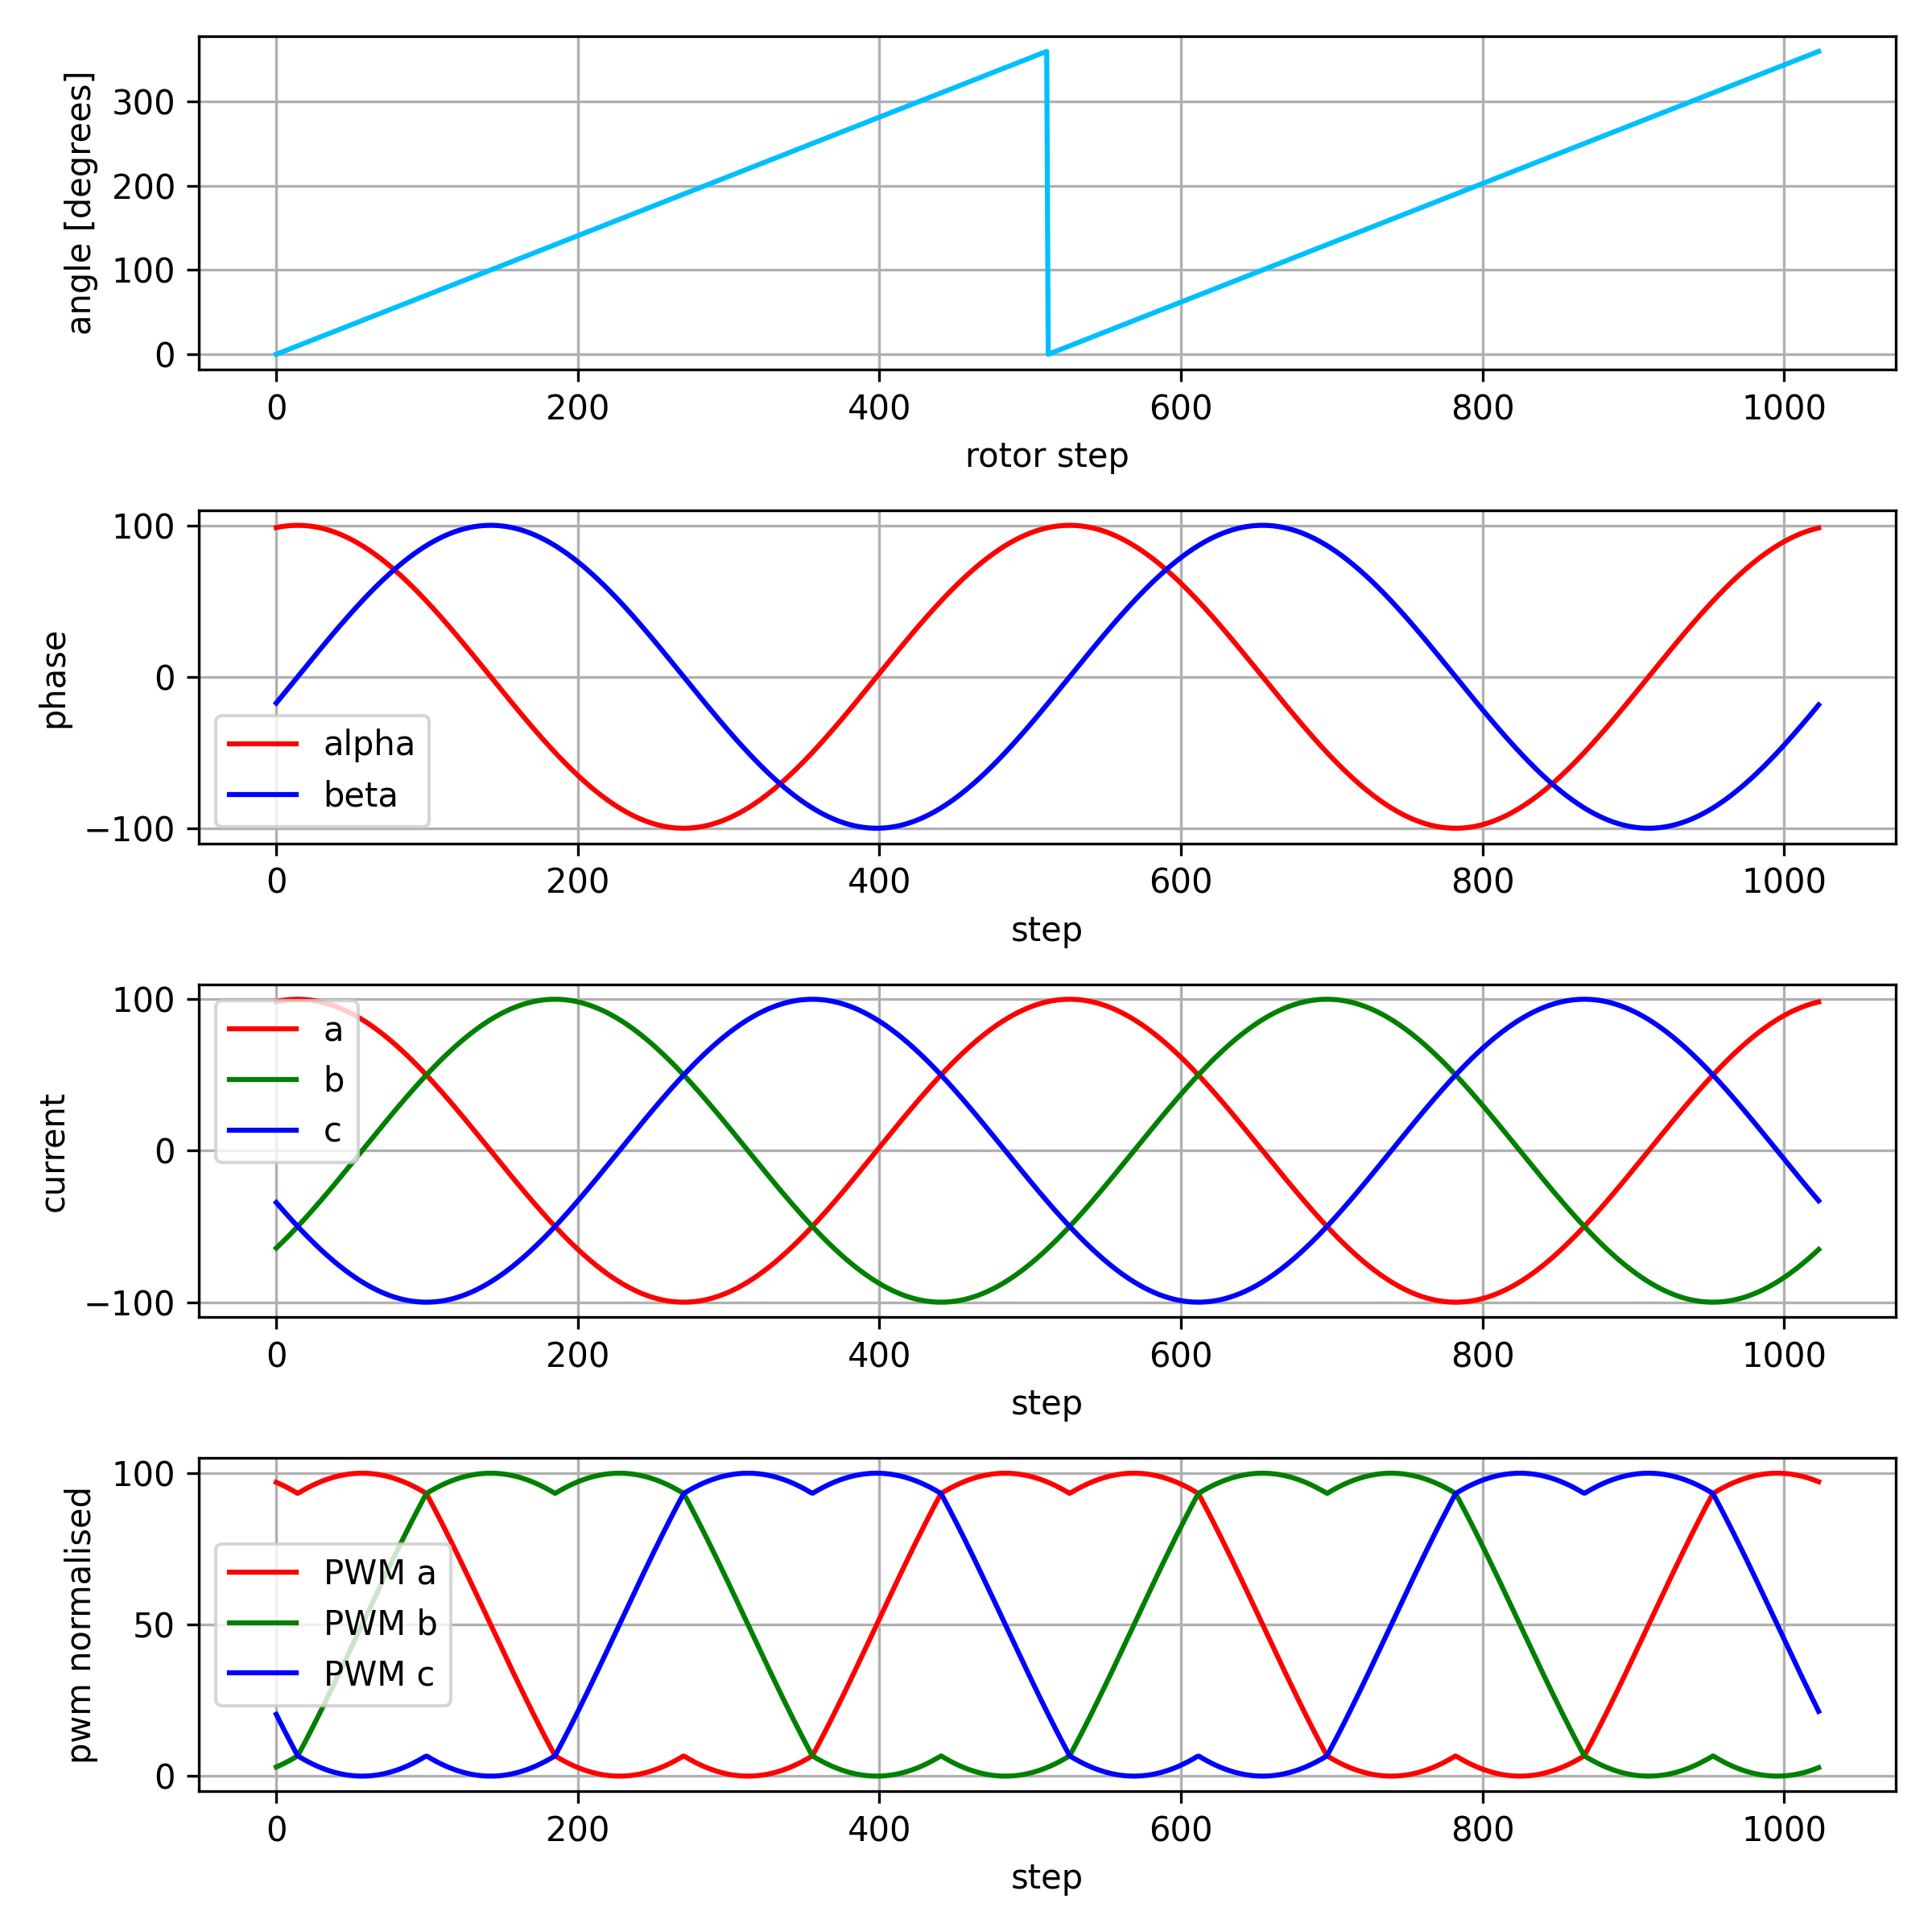
\includegraphics[scale=0.3]{../diagrams/controll/transformations.png}}
    \end{column}

    \begin{column}{0.5\textwidth}
      \centering{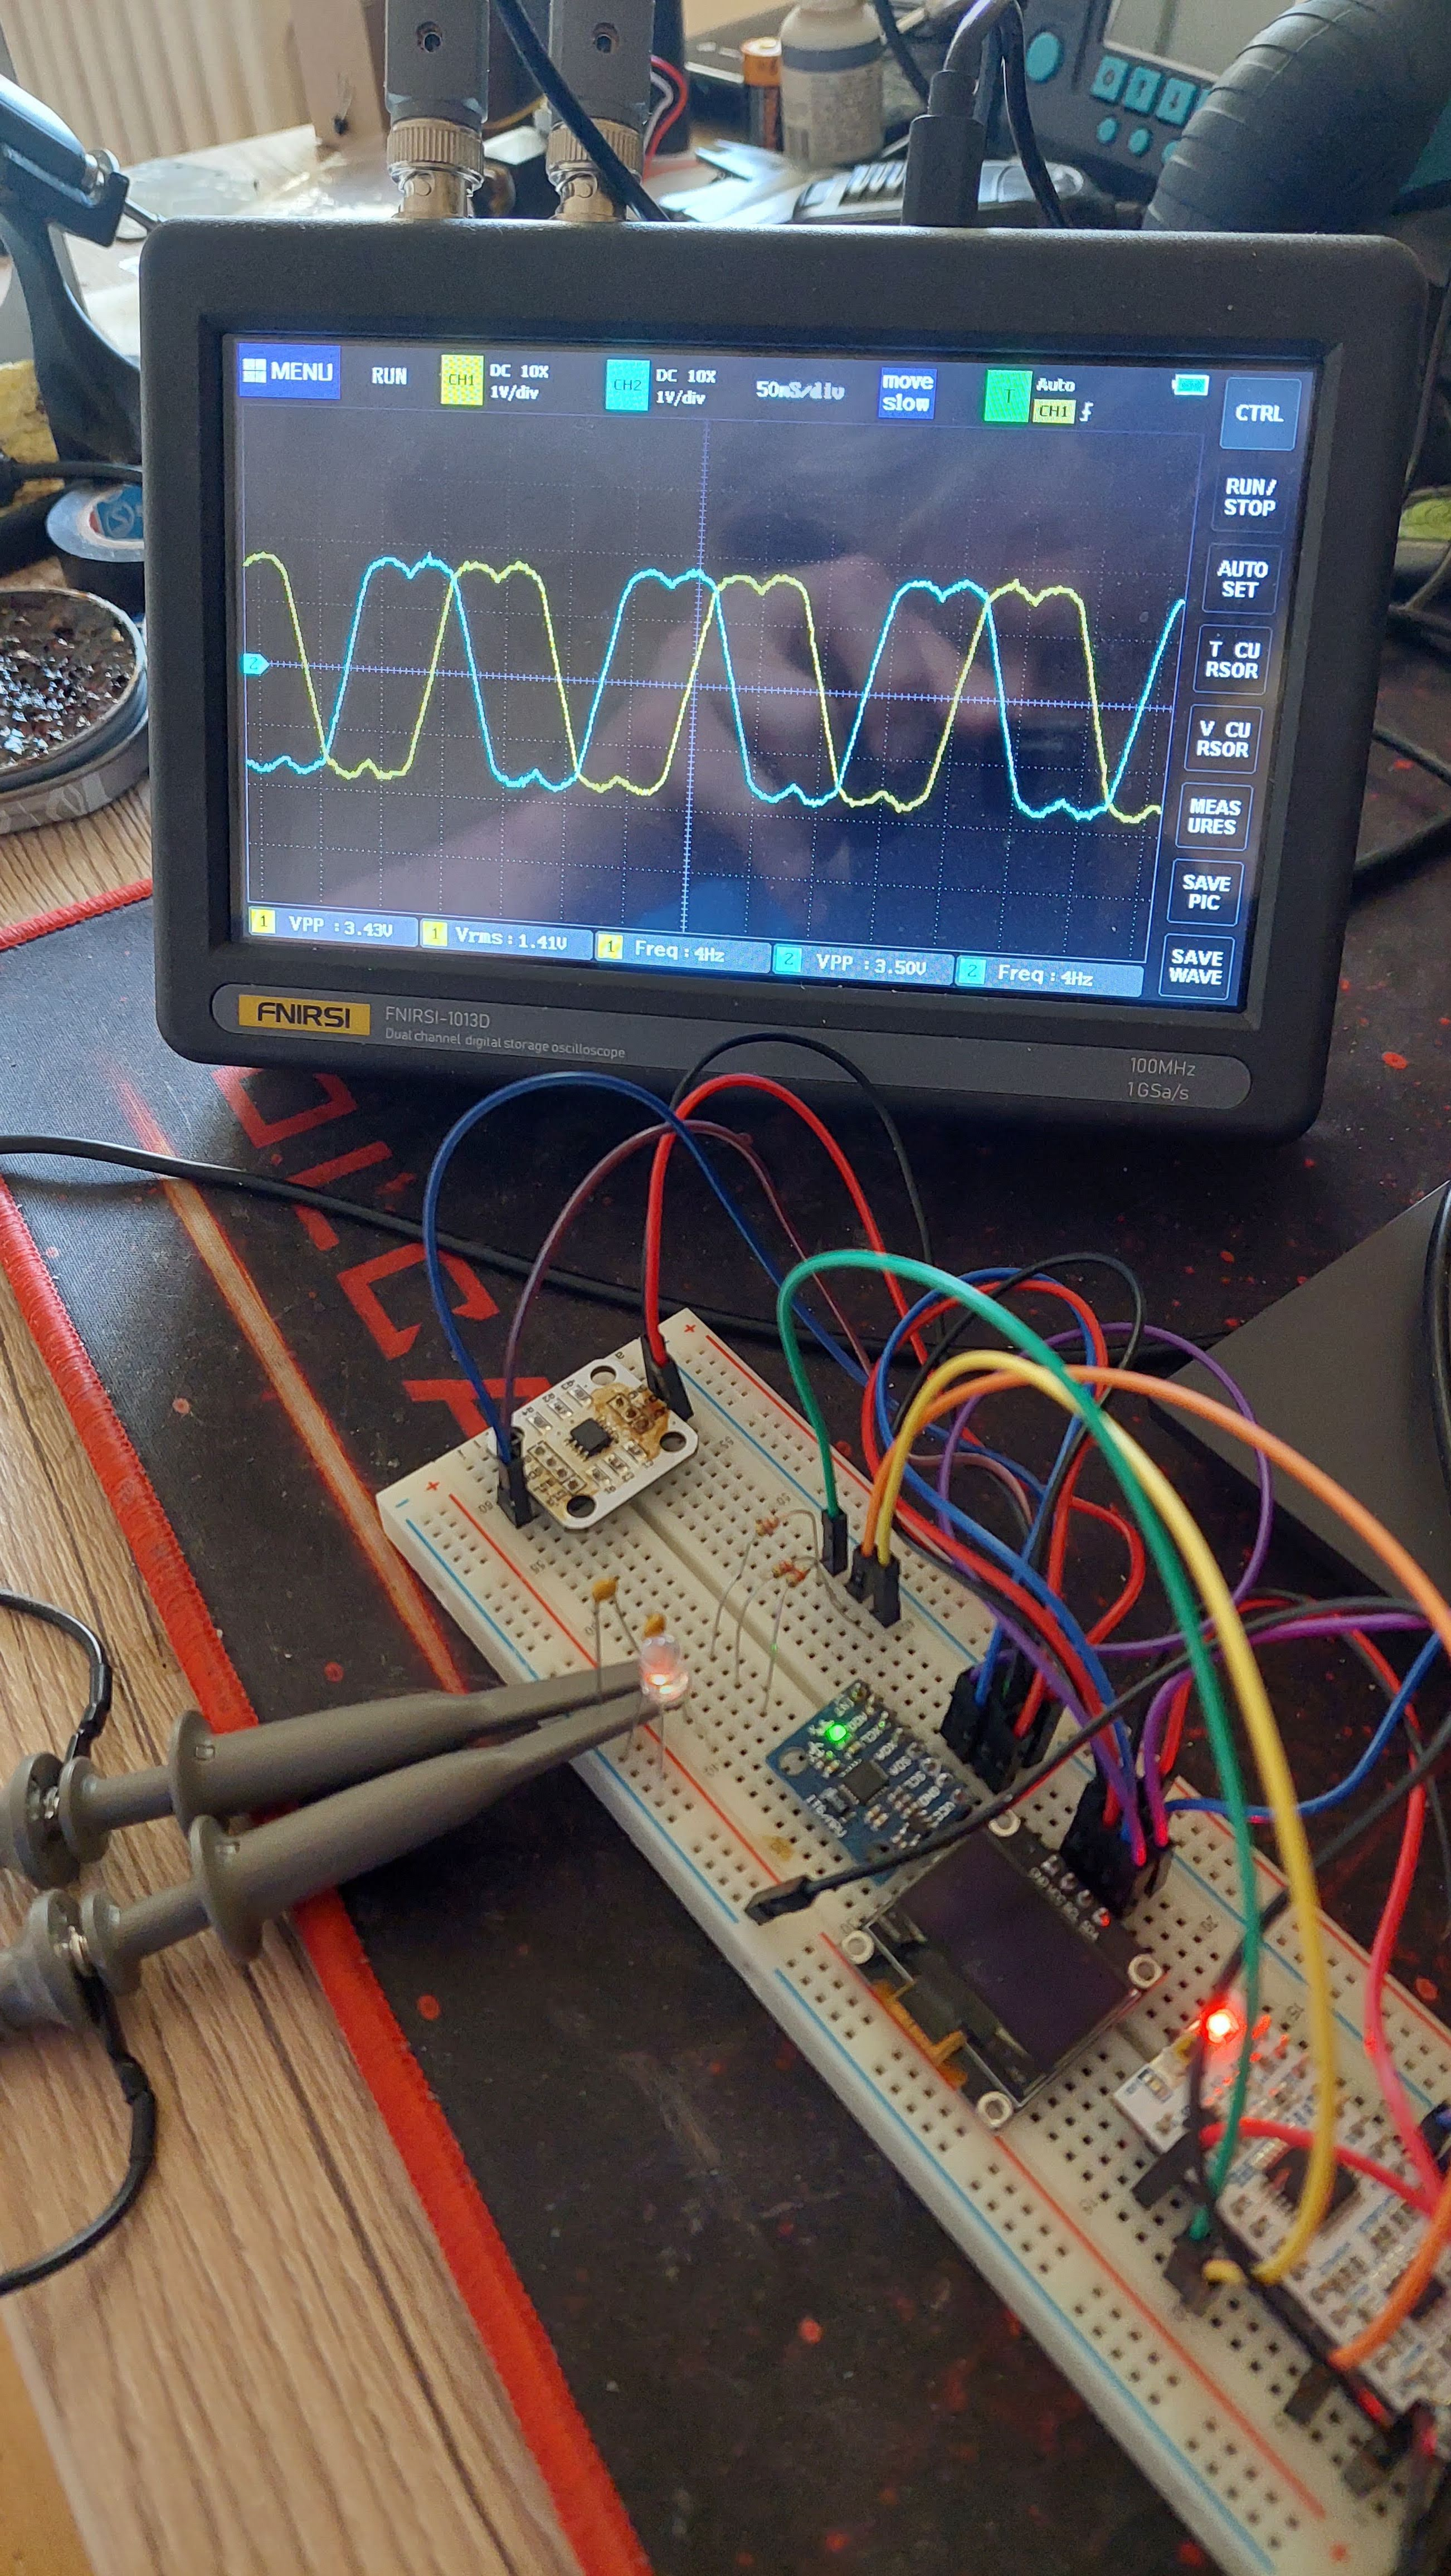
\includegraphics[scale=0.03]{../images/currents.jpg}}
    \end{column}

  \end{columns}

\end{frame}




\begin{frame}
  
  \frametitle{\bf image segmentation}    
  
    \begin{columns}

      \begin{column}{0.5\textwidth}
        \centering{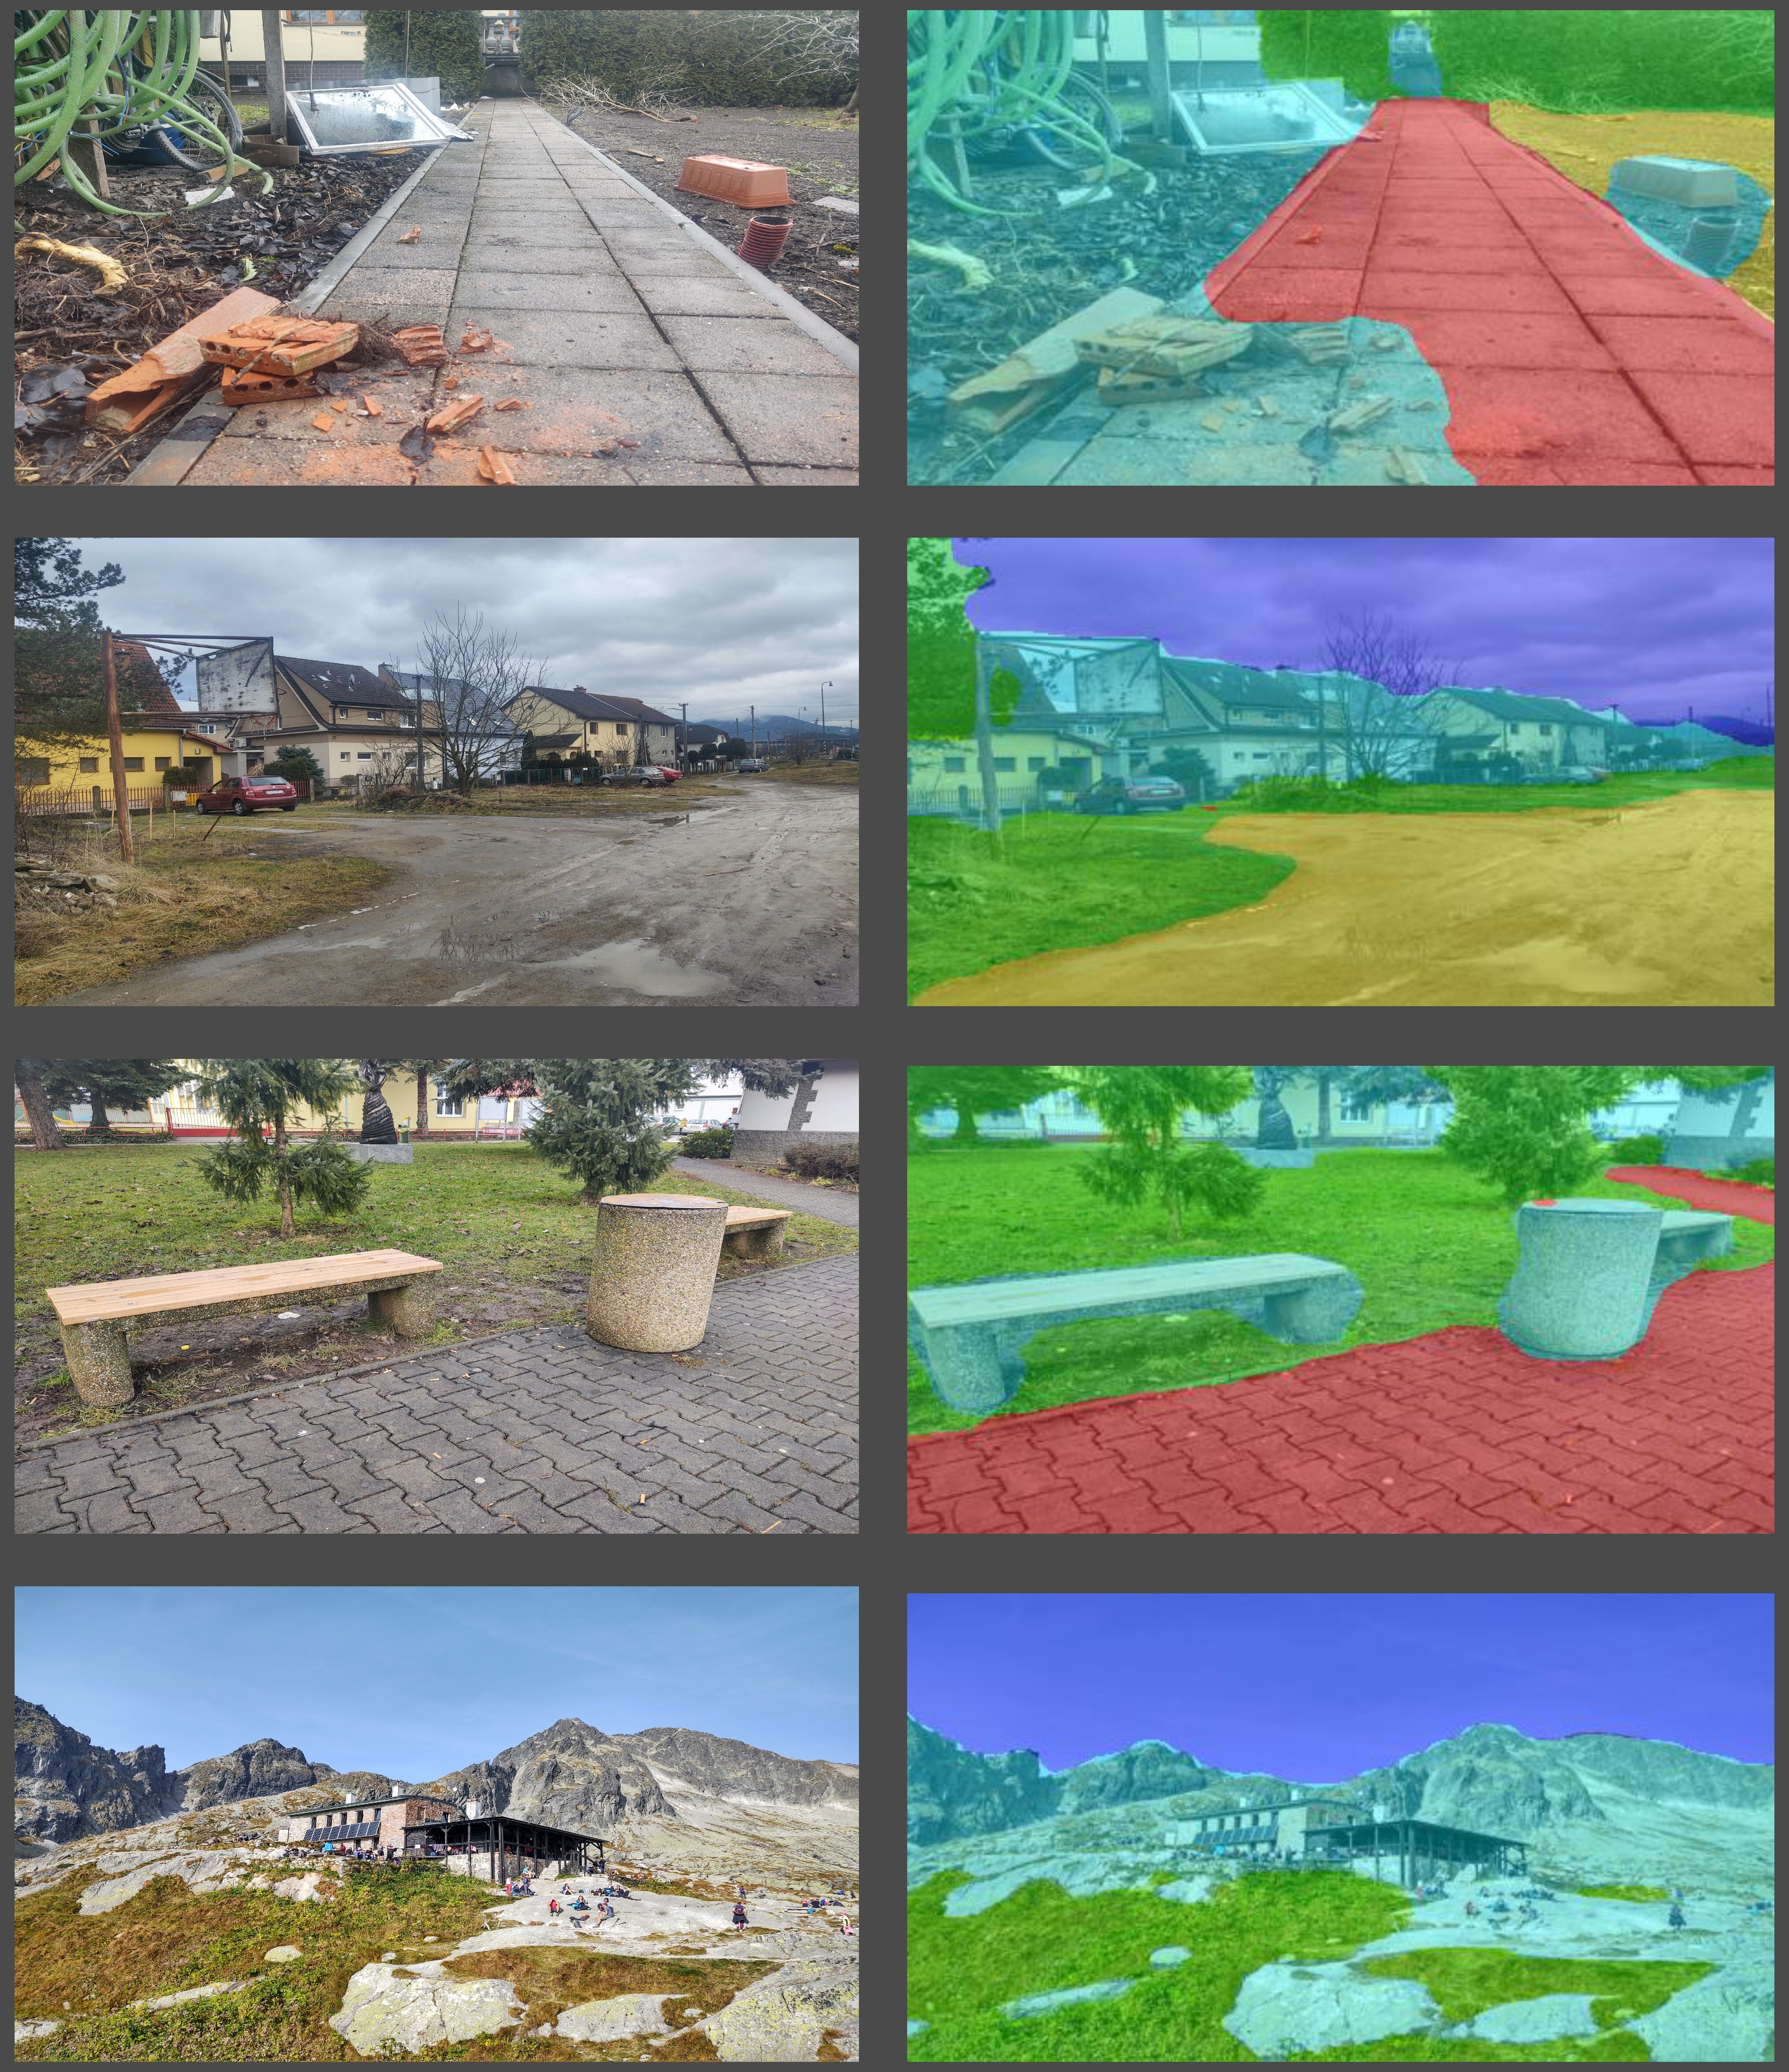
\includegraphics[scale=0.25]{../images/segmentation.jpg}}
      \end{column}

      \begin{column}{0.5\textwidth}
        \begin{itemize}
          \item deep learning
          \item convolutional neural networks
          \item resnet18, resnet50, u-net, mask2former ...
        \end{itemize}
      \end{column}

    \end{columns}

\end{frame}


\begin{frame}
  
  \frametitle{\bf convolutional neural network}    

    \centering{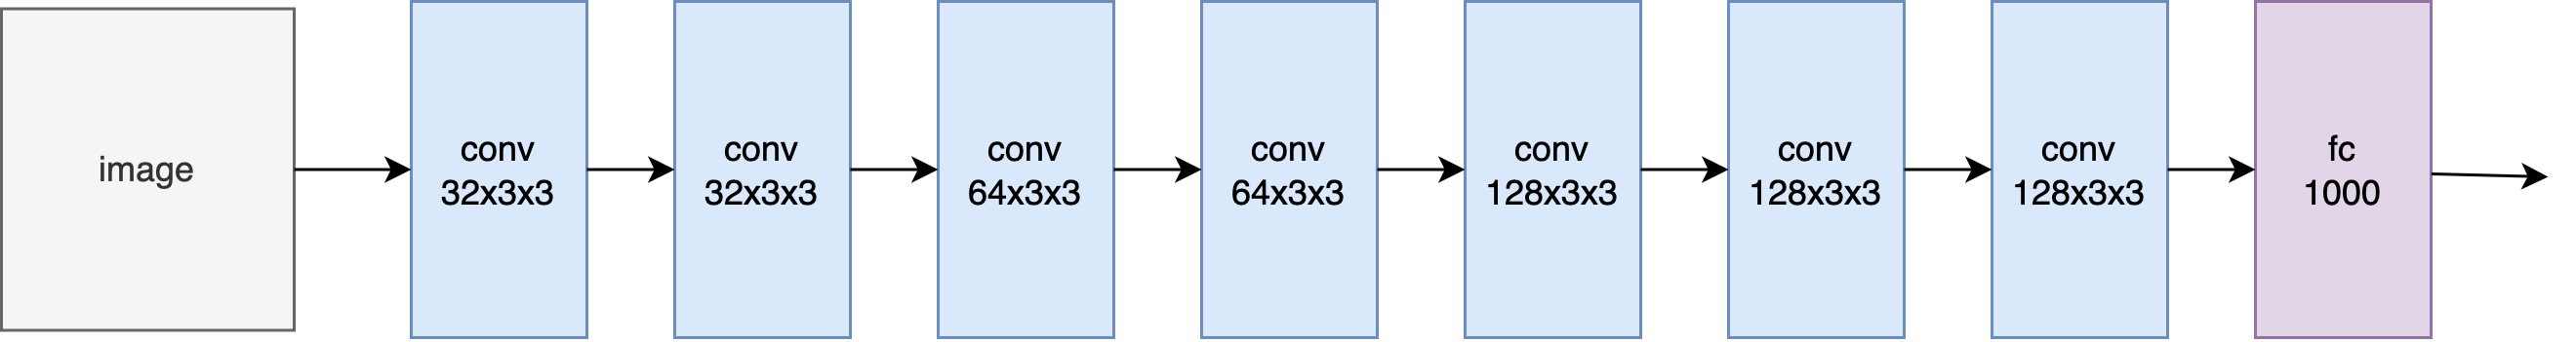
\includegraphics[scale=0.5]{../diagrams/models/models-simple_conv.png}}
  
    \begin{itemize}
      \item use 3x3 kernels
      \item strides instead of poolings
      \item ReLU activation
      \item Adam optimizer
    \end{itemize}
\end{frame}


\begin{frame}
  
  \frametitle{\bf resnet}    

    \centering{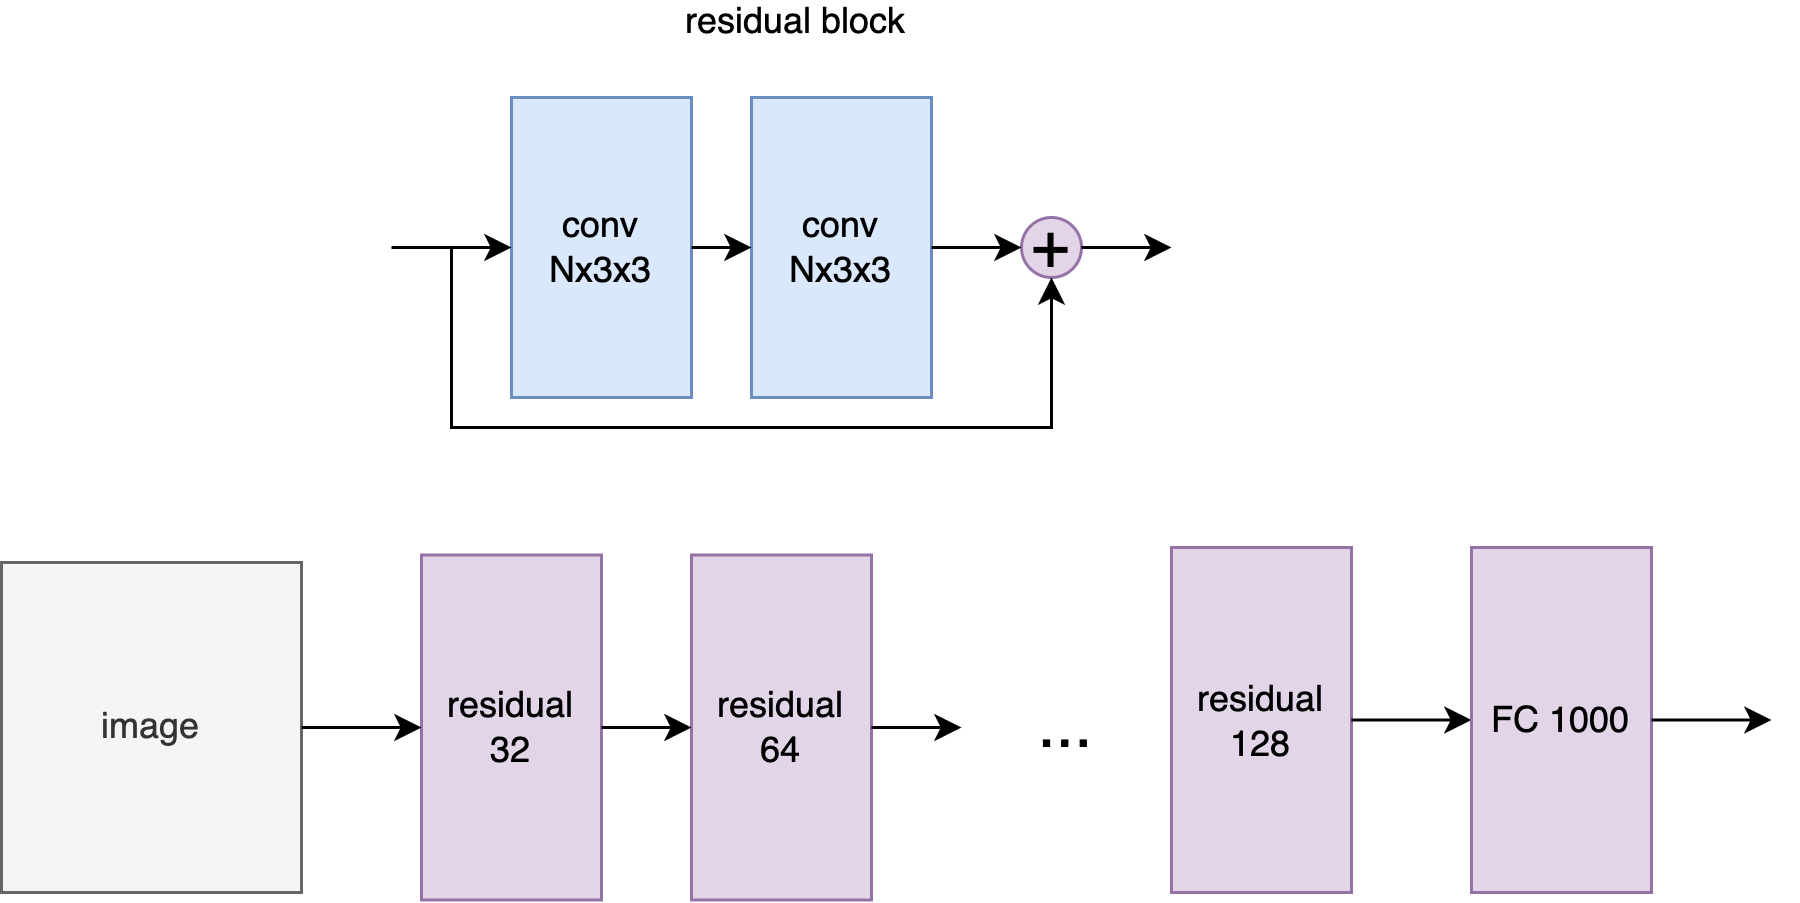
\includegraphics[scale=0.5]{../diagrams/models/models-resnet.png}}
  
    \begin{itemize}
      \item skip connections
      \item resnet18, 50, 110
      \item AlphaGO, AlphaZero
    \end{itemize}
\end{frame}


\begin{frame}
  
  \frametitle{\bf segmentation}    

    \centering{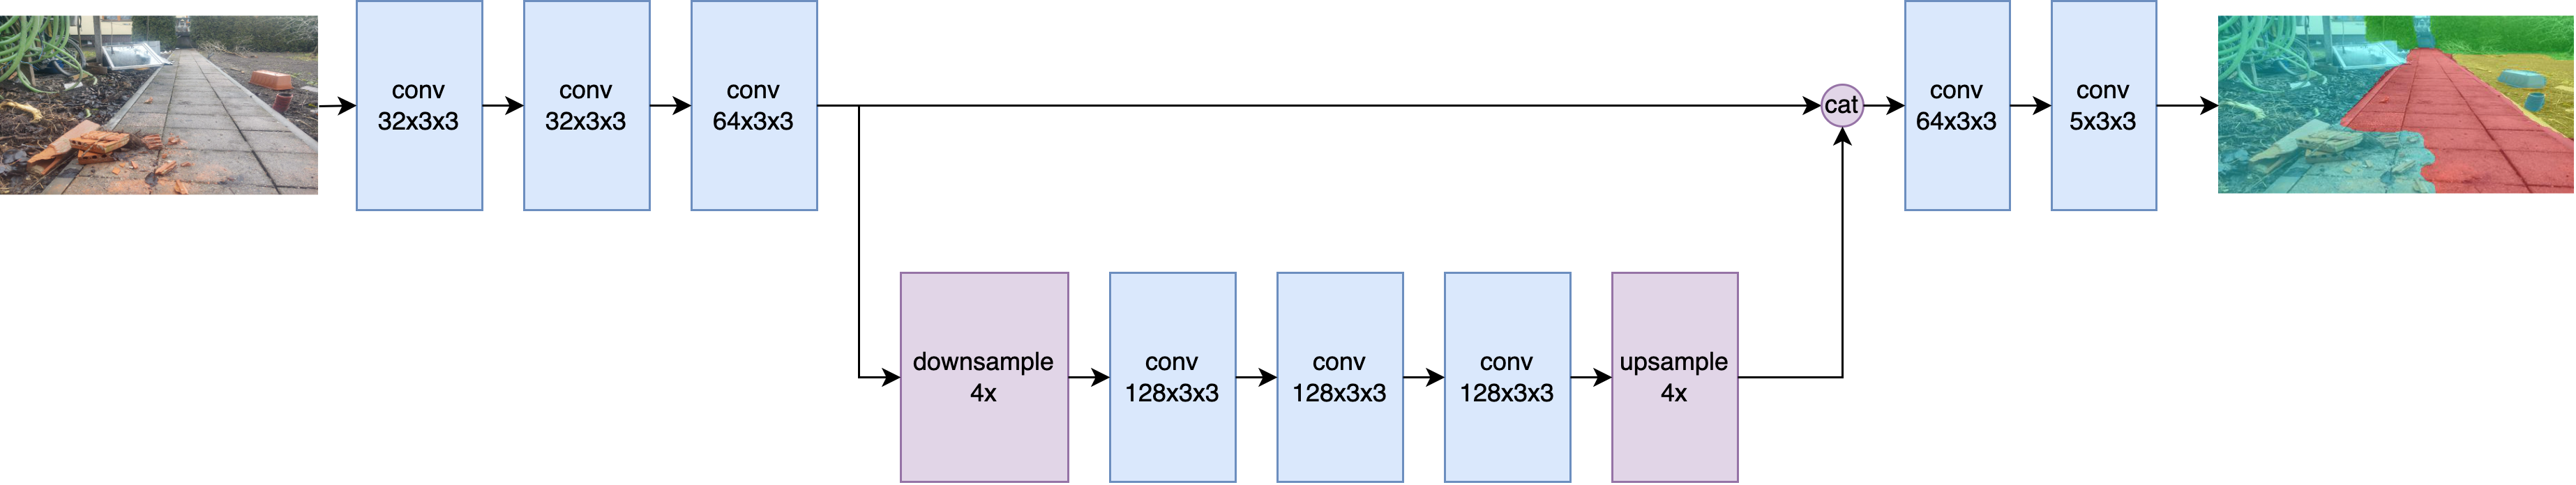
\includegraphics[scale=0.35]{../diagrams/models/models-segmentation.png}}
  
    \begin{itemize}
      \item multiple sizes views
      \item 10FPS on NVIDIA jetson nano
    \end{itemize}
\end{frame}





\begin{frame}{\bf reinforcement learning}

  \begin{columns}

    \begin{column}{0.5\textwidth}
      \centering{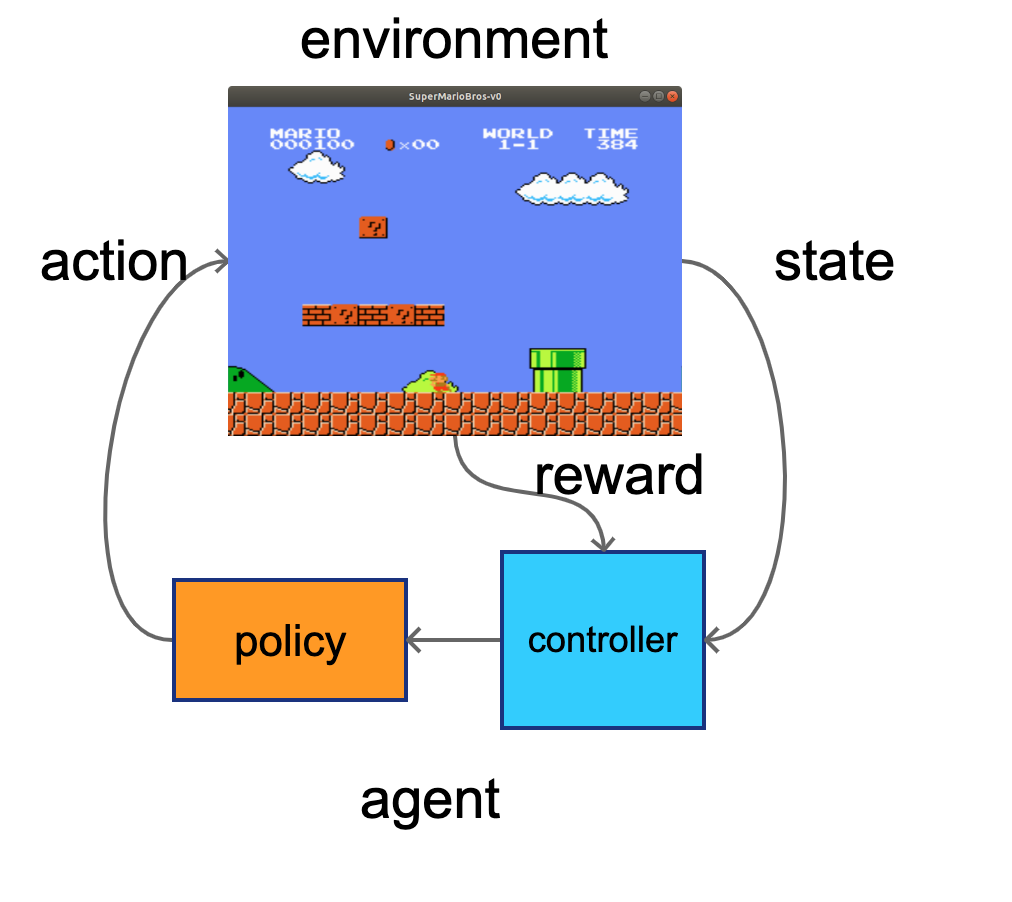
\includegraphics[scale=0.15]{../diagrams/basic/reinforcementlearning.png}}
    \end{column}

    \begin{column}{0.5\textwidth}
      \begin{itemize}
        \item obtain state
        \item select action
        \item exectute action
        \item learn from experiences
      \end{itemize}
    \end{column}

  \end{columns}

\end{frame}





\begin{frame}{\bf deep reinforcement learning - playing Atari}

  \begin{columns}

    \begin{column}{0.5\textwidth}
      \centering{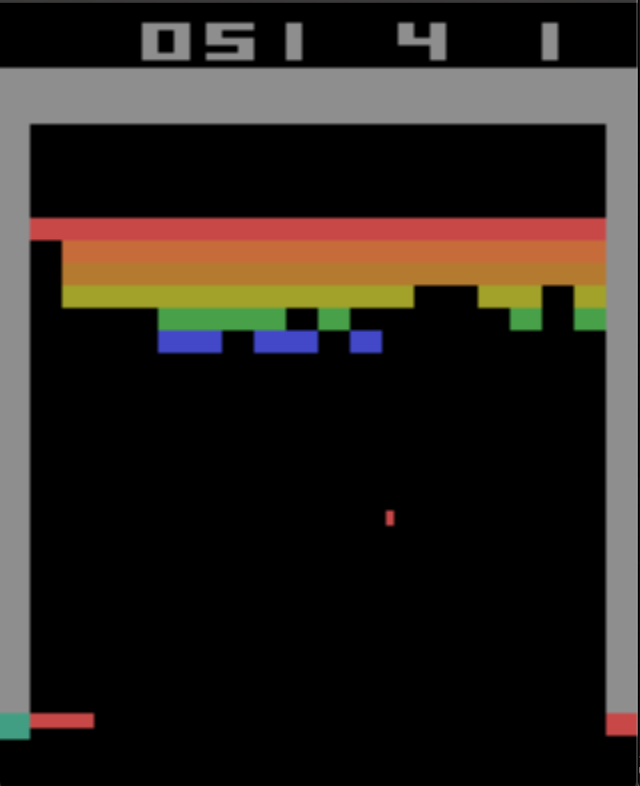
\includegraphics[scale=0.35]{../images/breakout.png}}
    \end{column}

    \begin{column}{0.5\textwidth}
      \centering{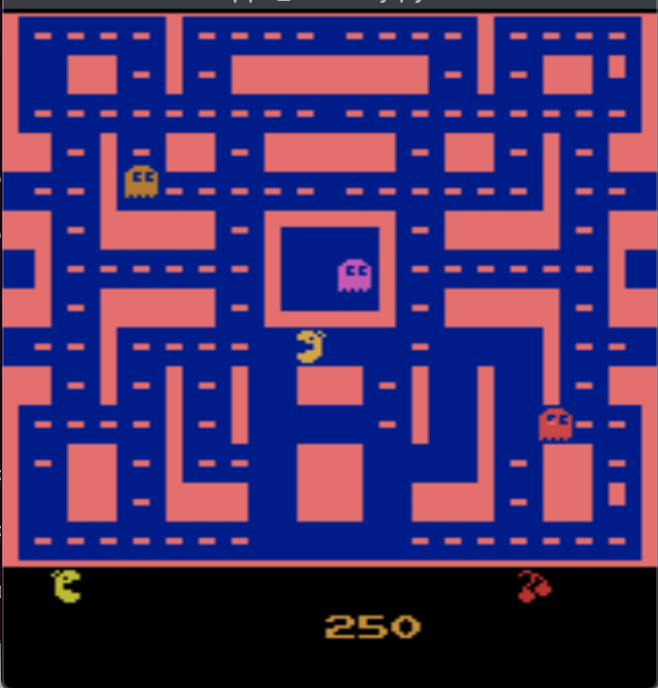
\includegraphics[scale=0.3]{../images/pacman.png}}
    \end{column}

  \end{columns}

  2013, Mnih (DeepMind) : Playing Atari with Deep Reinforcement Learning, 
  \url{https://arxiv.org/pdf/1312.5602.pdf}
\end{frame}


\begin{frame}{\bf reinforcement learning - path to superhuman score}

  \begin{columns}

    \begin{column}{0.5\textwidth}
      \centering{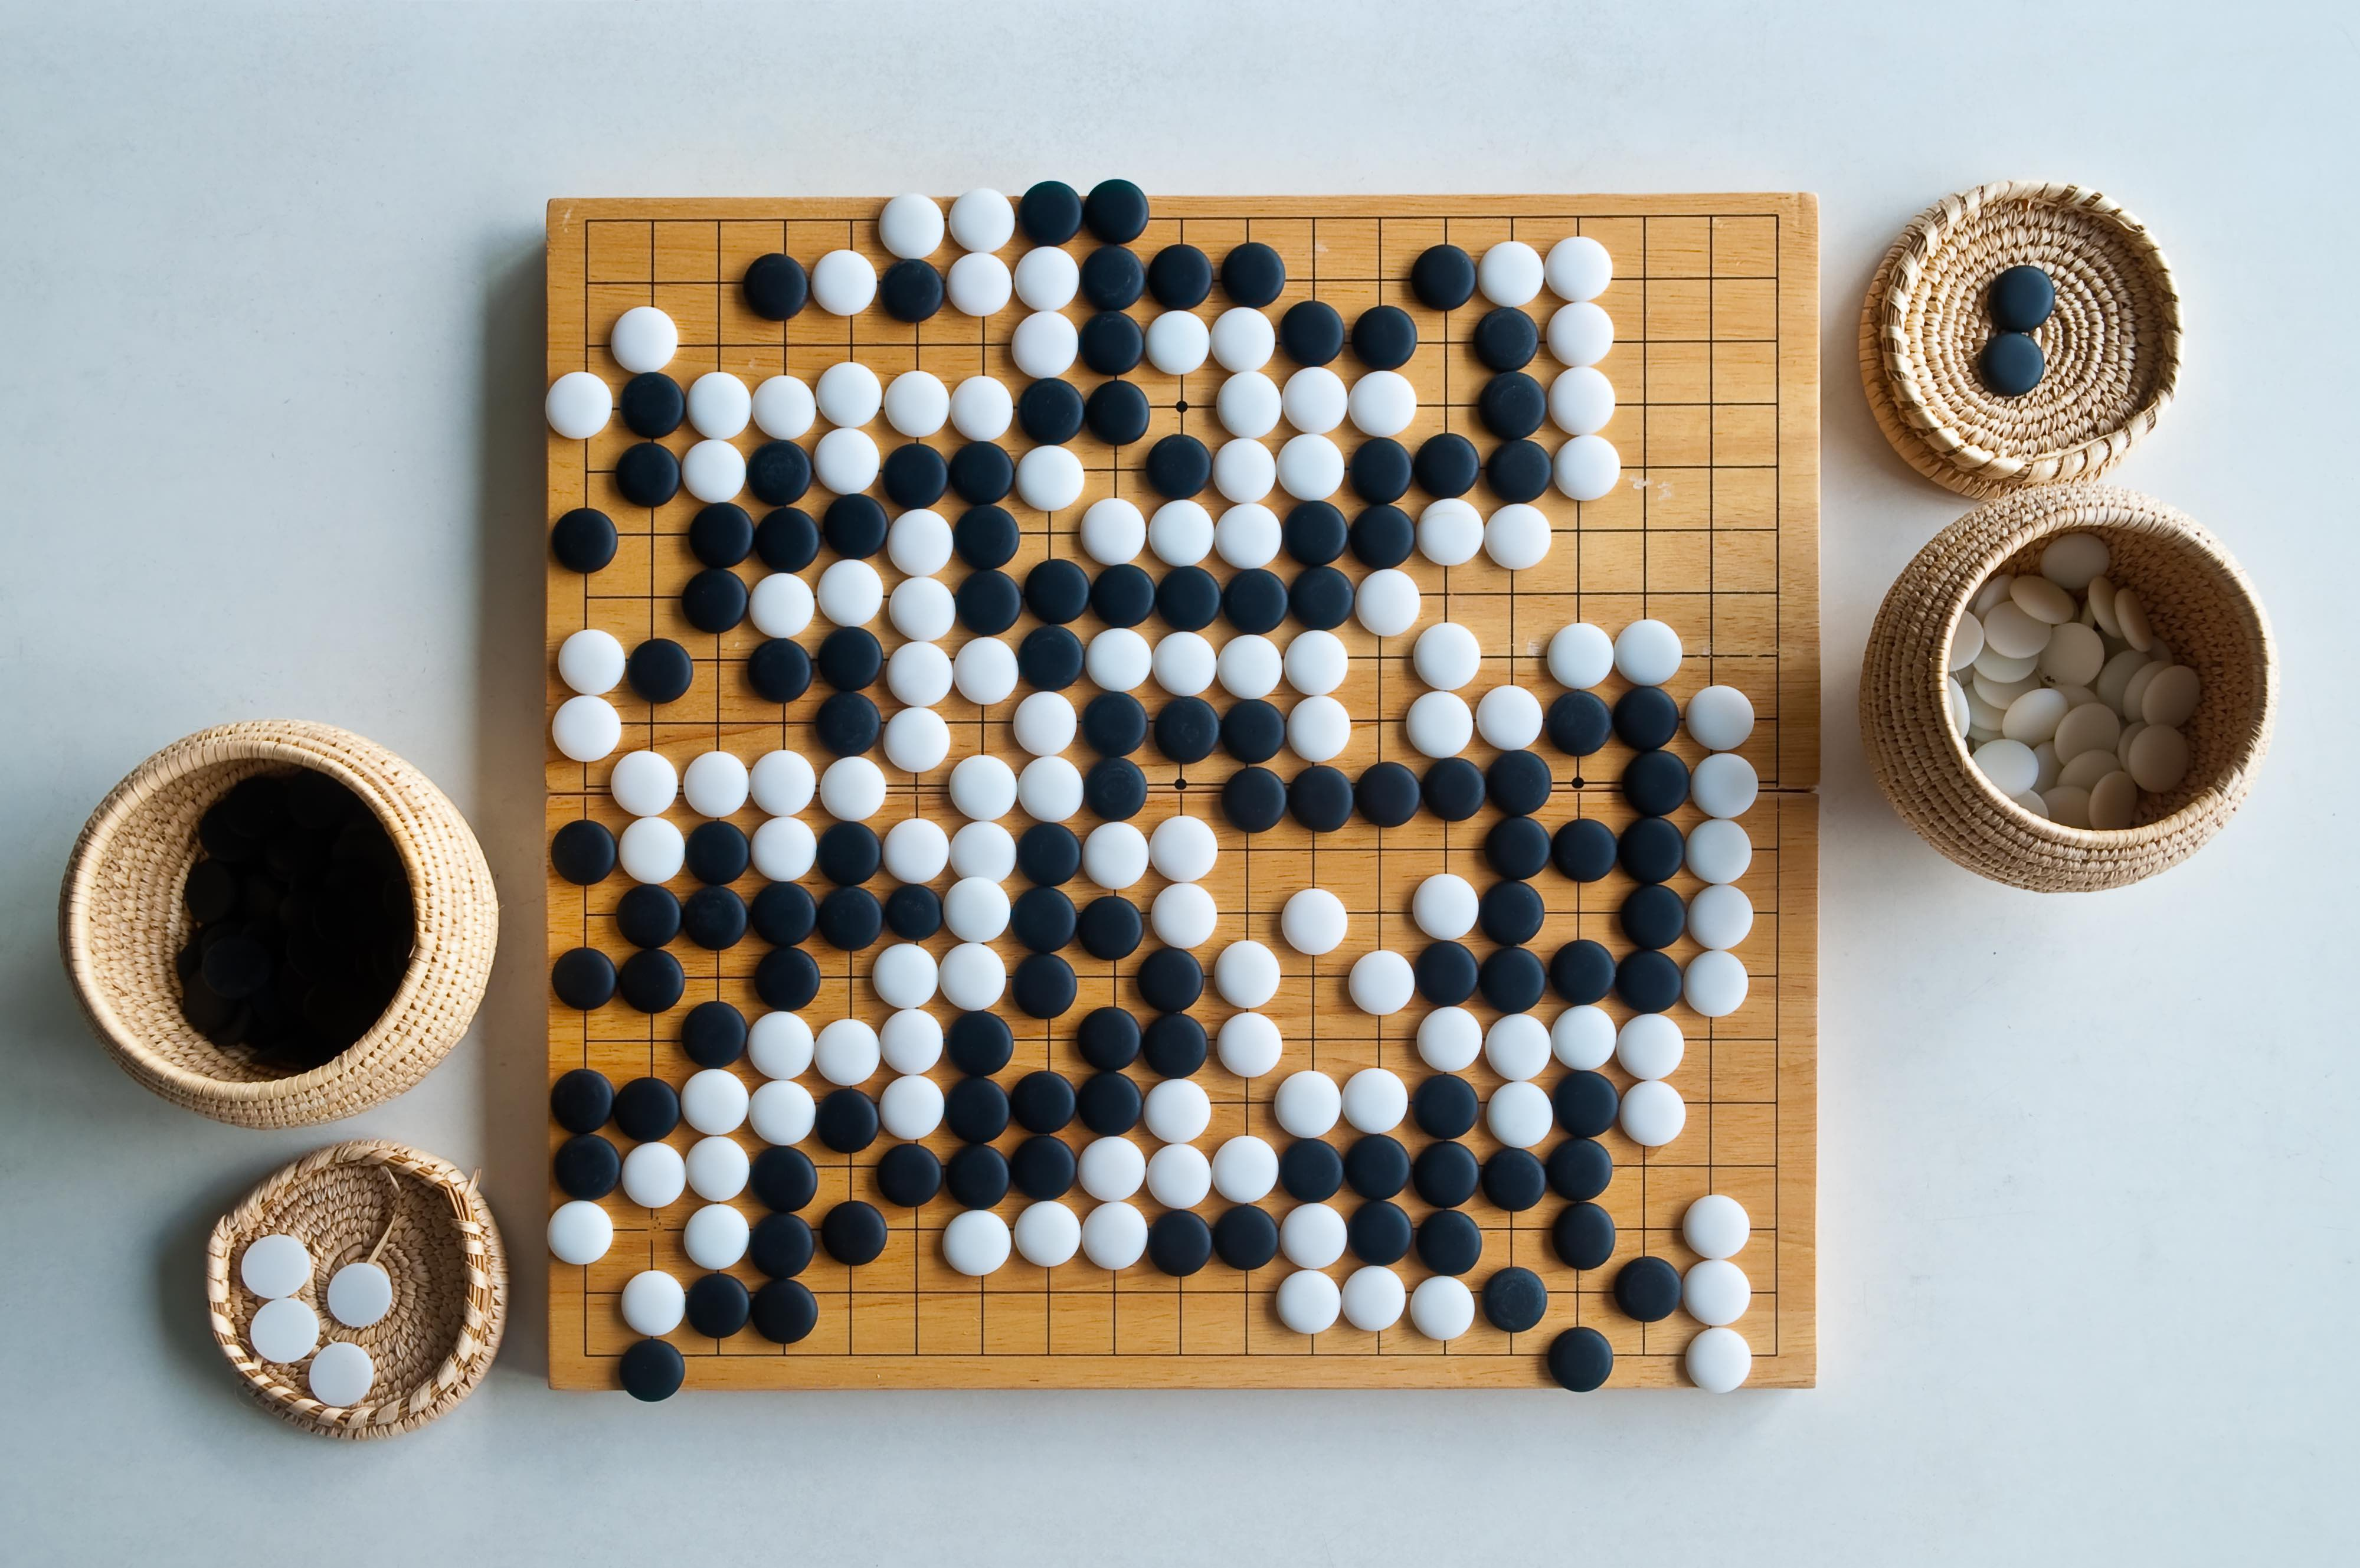
\includegraphics[scale=0.03]{../images/go.jpg}}
    \end{column}

    \begin{column}{0.5\textwidth}
      \centering{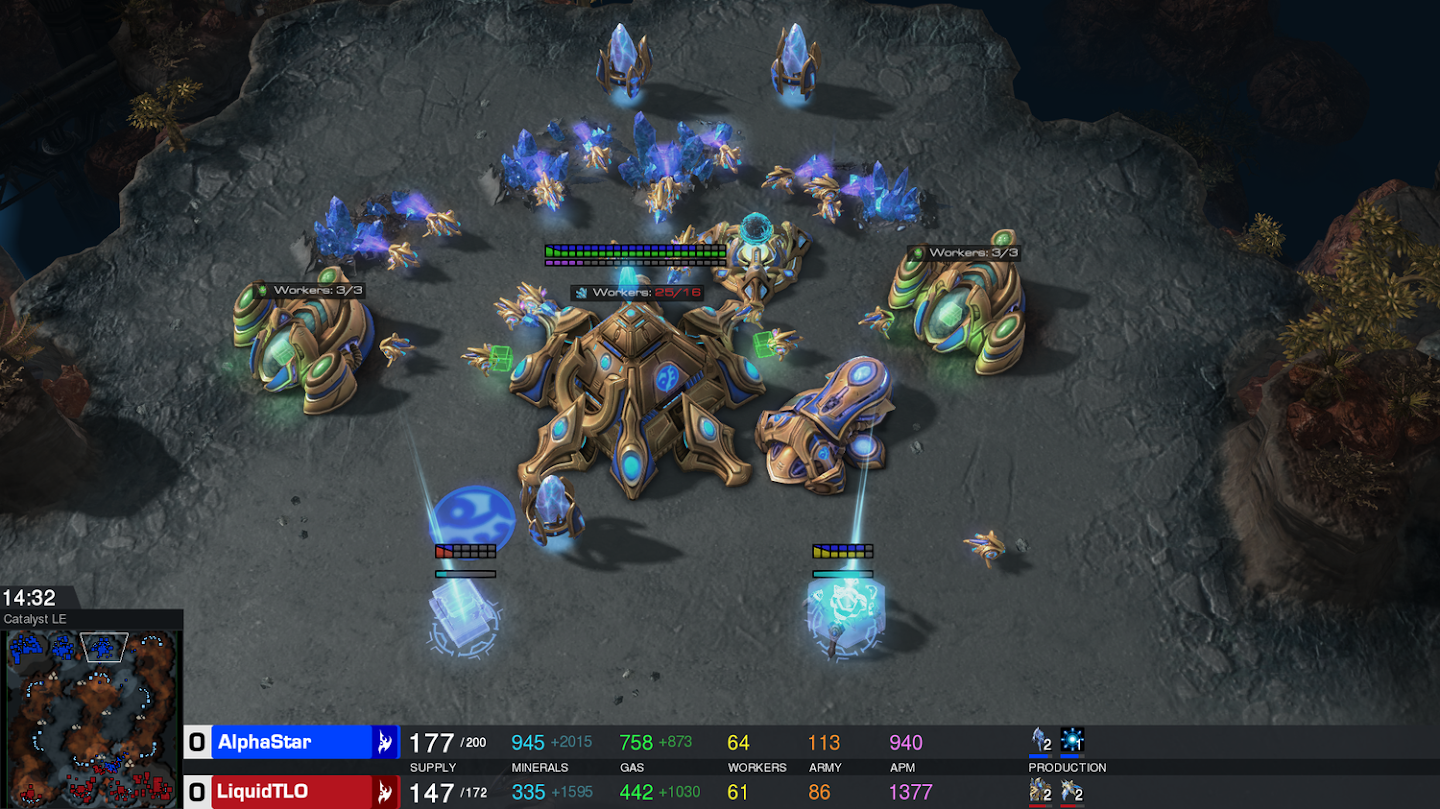
\includegraphics[scale=0.1]{../images/starcraft.png}}
    \end{column}

  \end{columns}

  \begin{itemize} 
    \item 2016 AlphaGo, \url{https://www.nature.com/articles/nature16961}
    \item 2020 MuZero, \url{https://arxiv.org/pdf/1911.08265.pdf}
    \item AlphaZero, AlphaStar ...
  \end{itemize}
\end{frame}

\begin{frame}{\bf reinforcement learning - robotics}

  \begin{columns}

    \begin{column}{0.5\textwidth}
      \centering{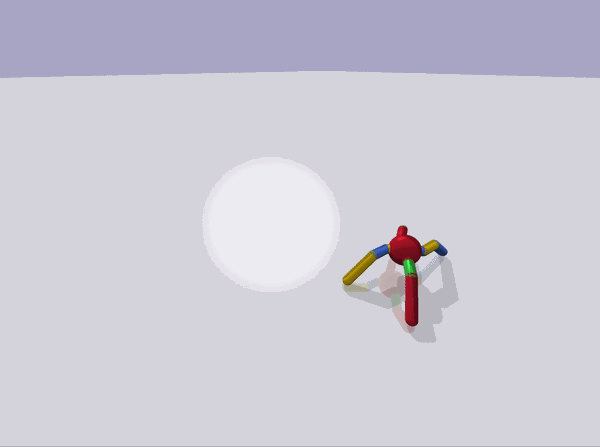
\includegraphics[scale=0.2]{../images/ant.png}}
      \centering{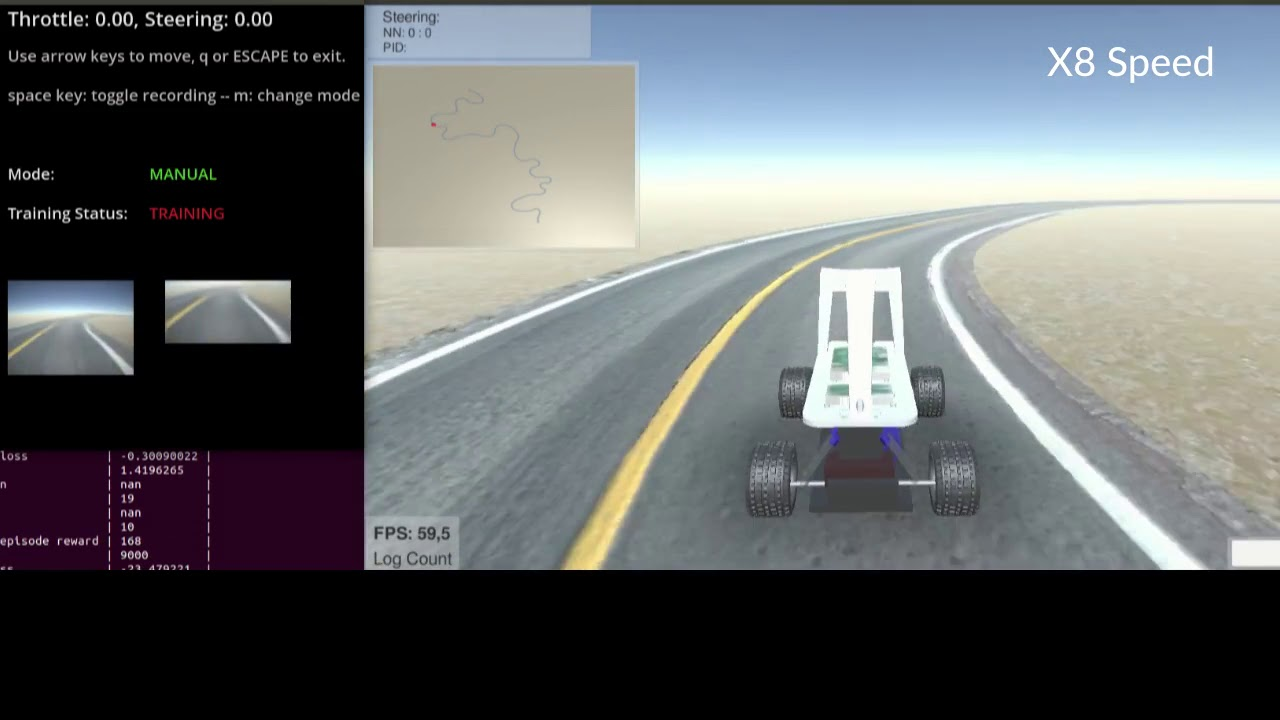
\includegraphics[scale=0.1]{../images/sac_car.jpg}}
    \end{column}

    \begin{column}{0.5\textwidth}
      \centering{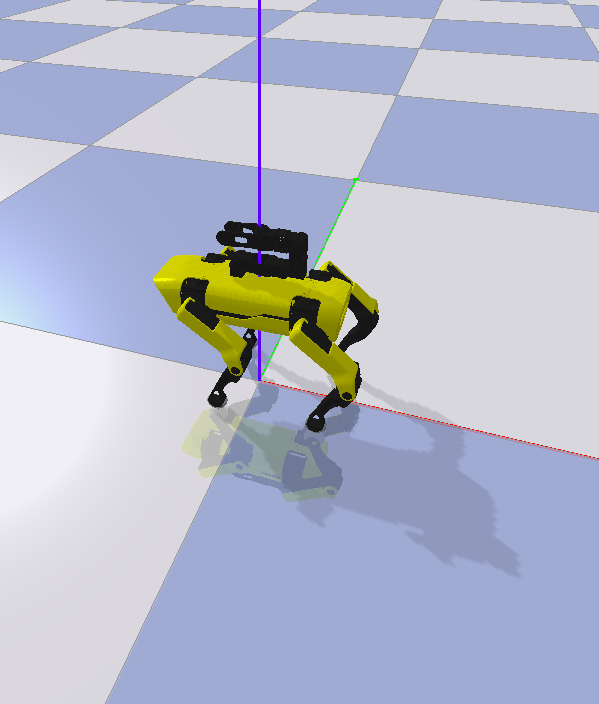
\includegraphics[scale=0.15]{../images/rex_arm.png}}
      \centering{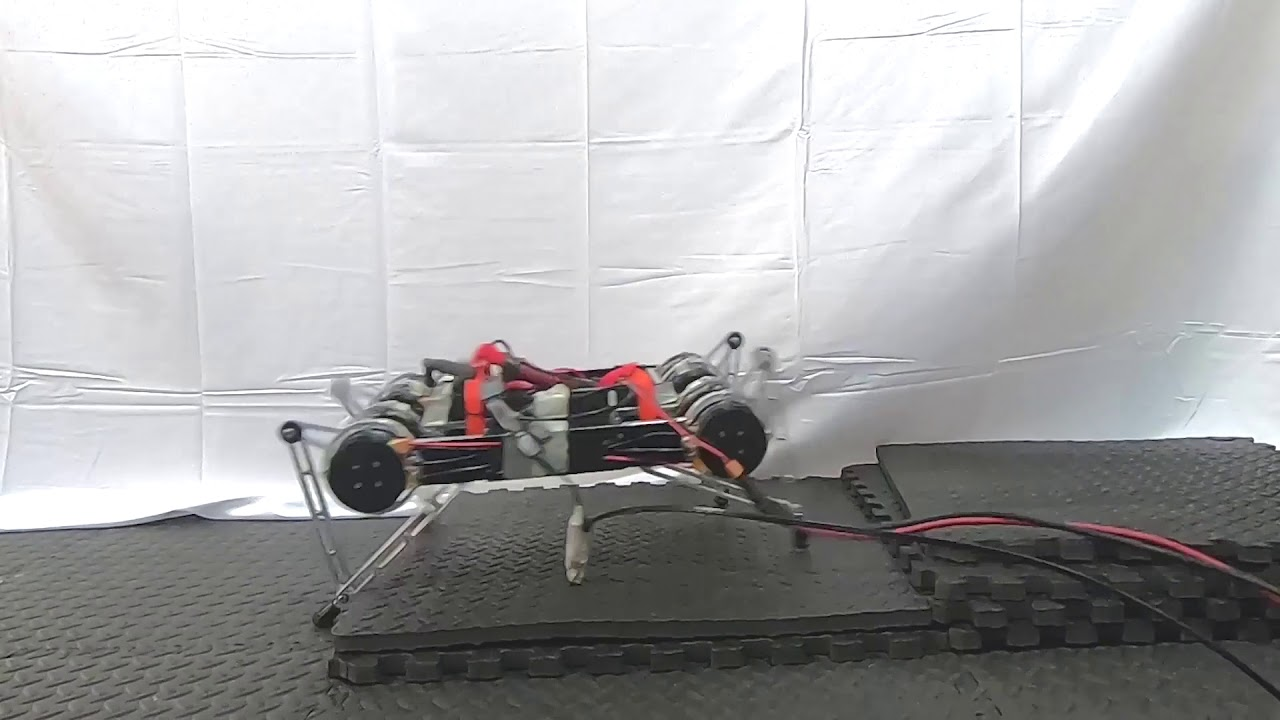
\includegraphics[scale=0.1]{../images/sac_minitaur.jpg}}
    \end{column}


  \end{columns}

\end{frame}


\begin{frame}{\bf motoko uprising - line follower}  
  \begin{columns}
    \begin{column}{0.5\textwidth}
      \centering{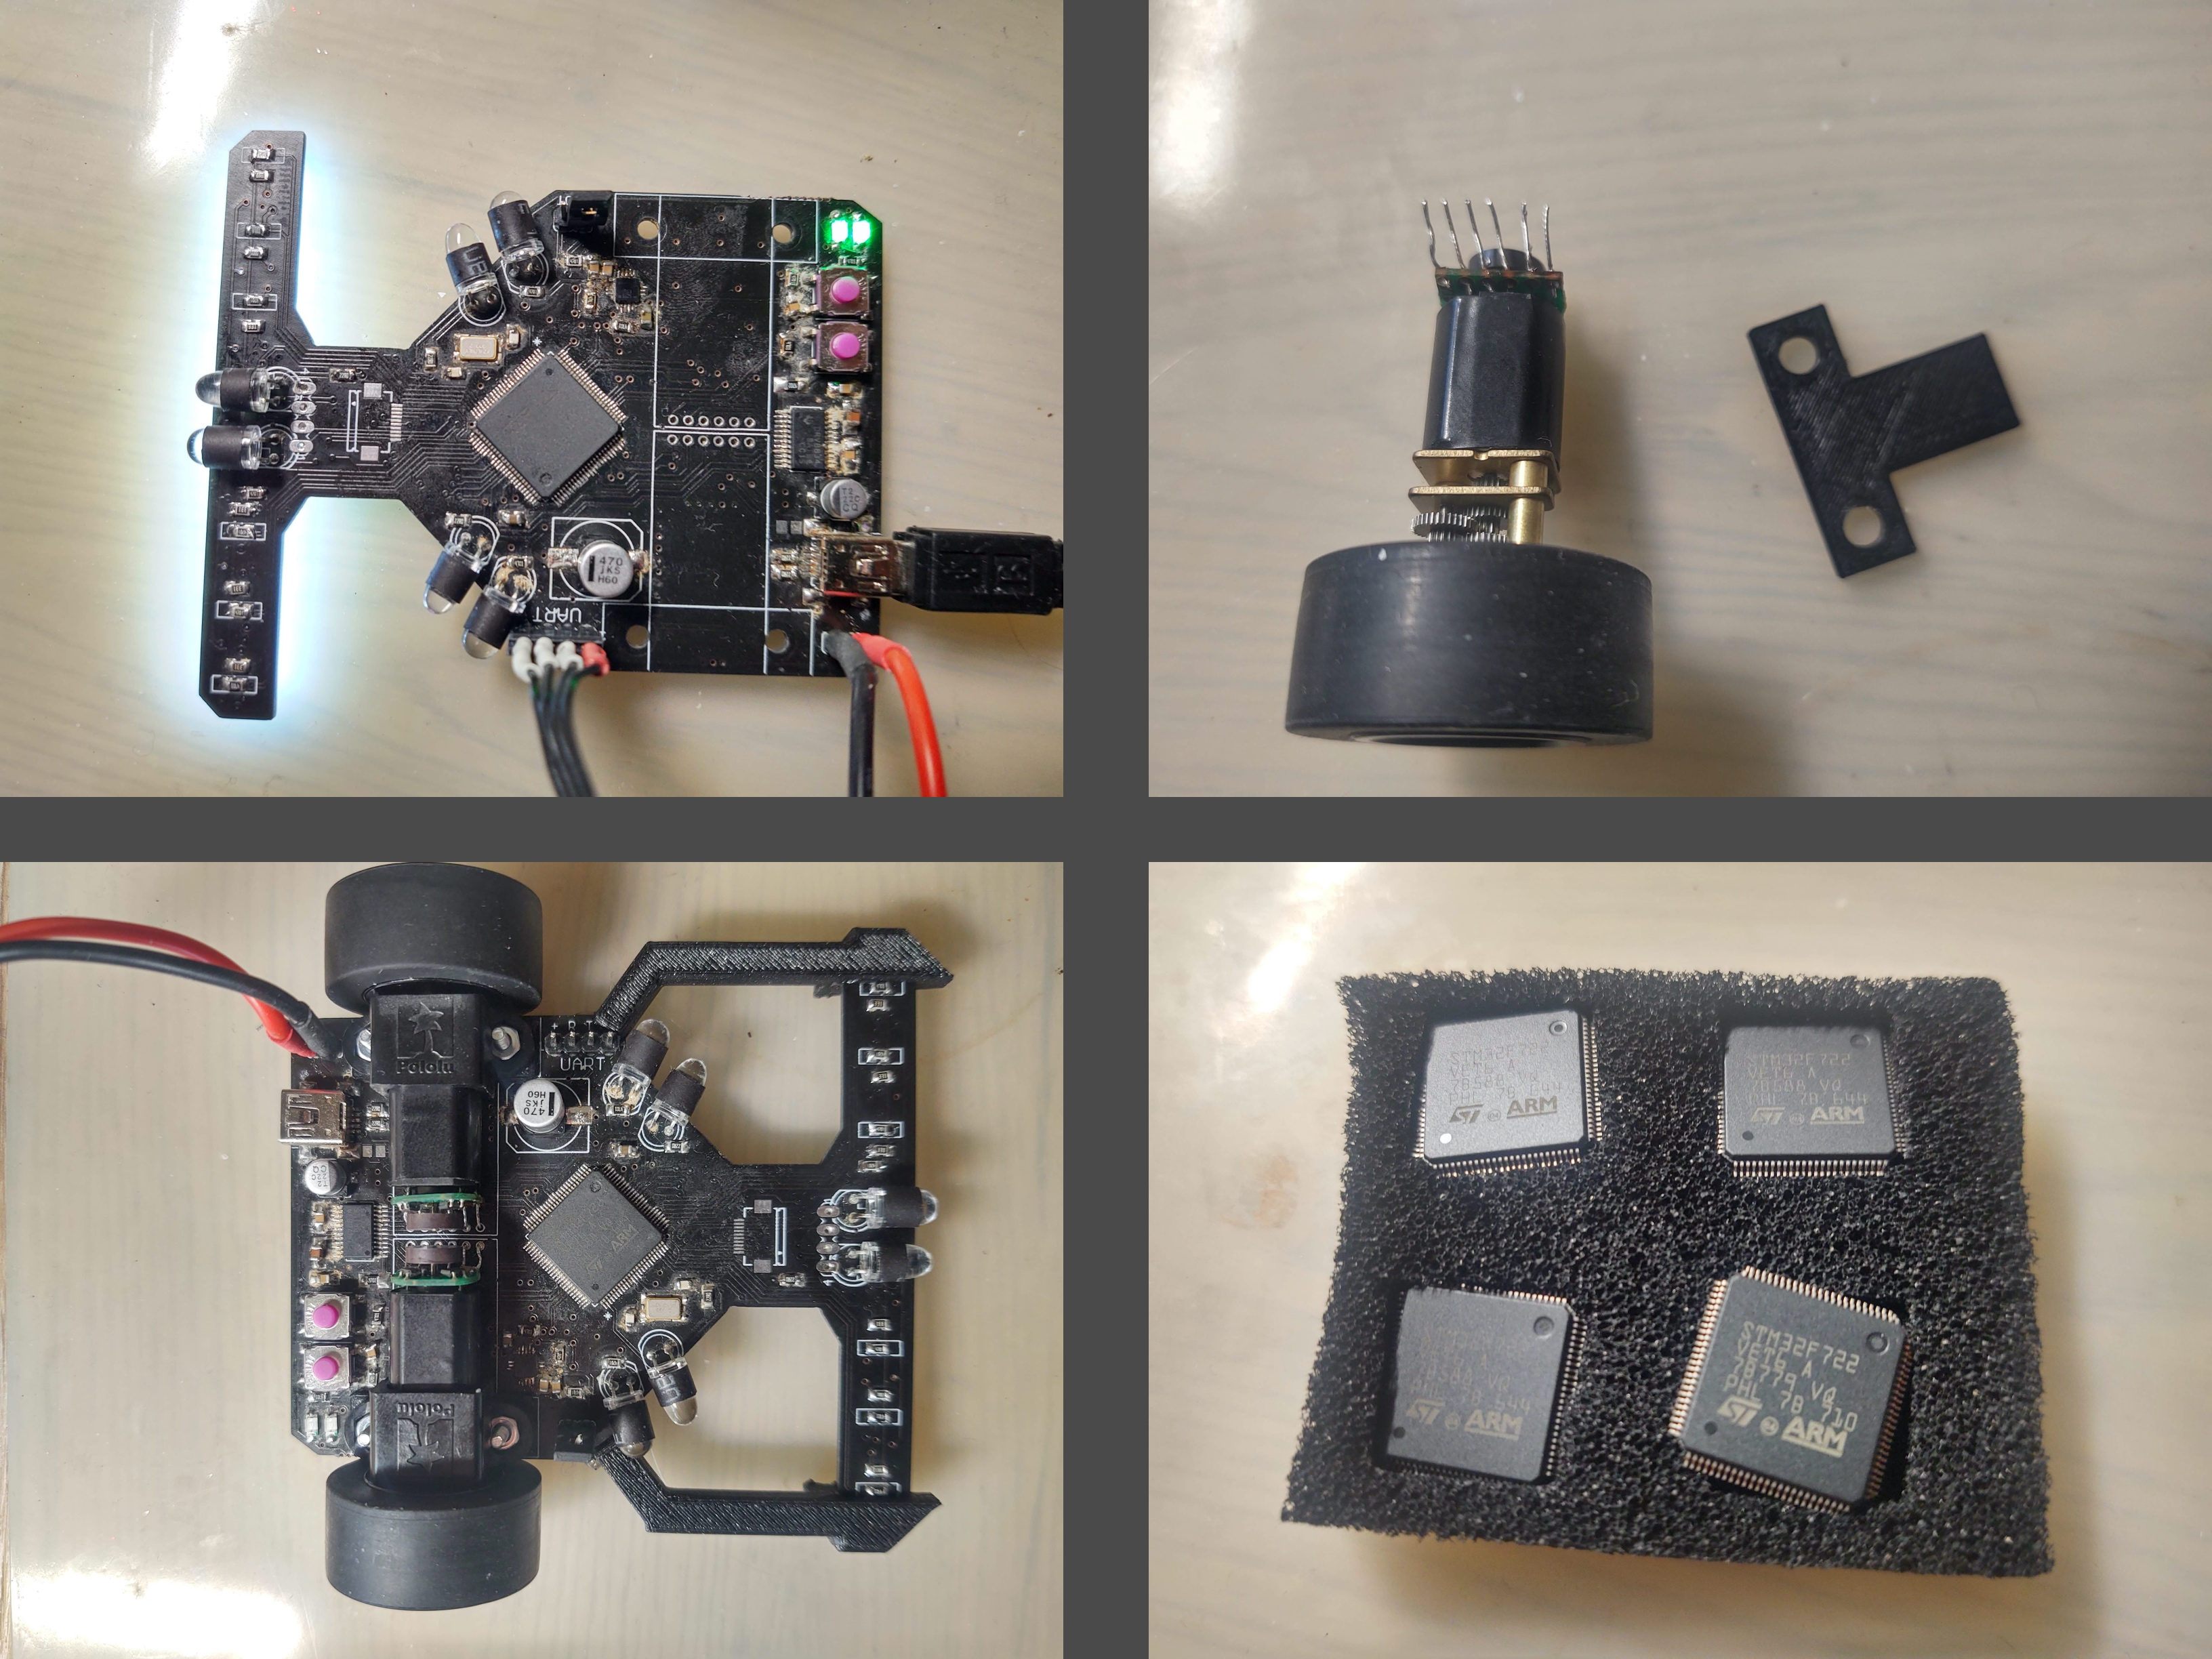
\includegraphics[scale=0.2]{../images/robot_mount.jpg}}
    \end{column}

    \begin{column}{0.5\textwidth}
      \centering{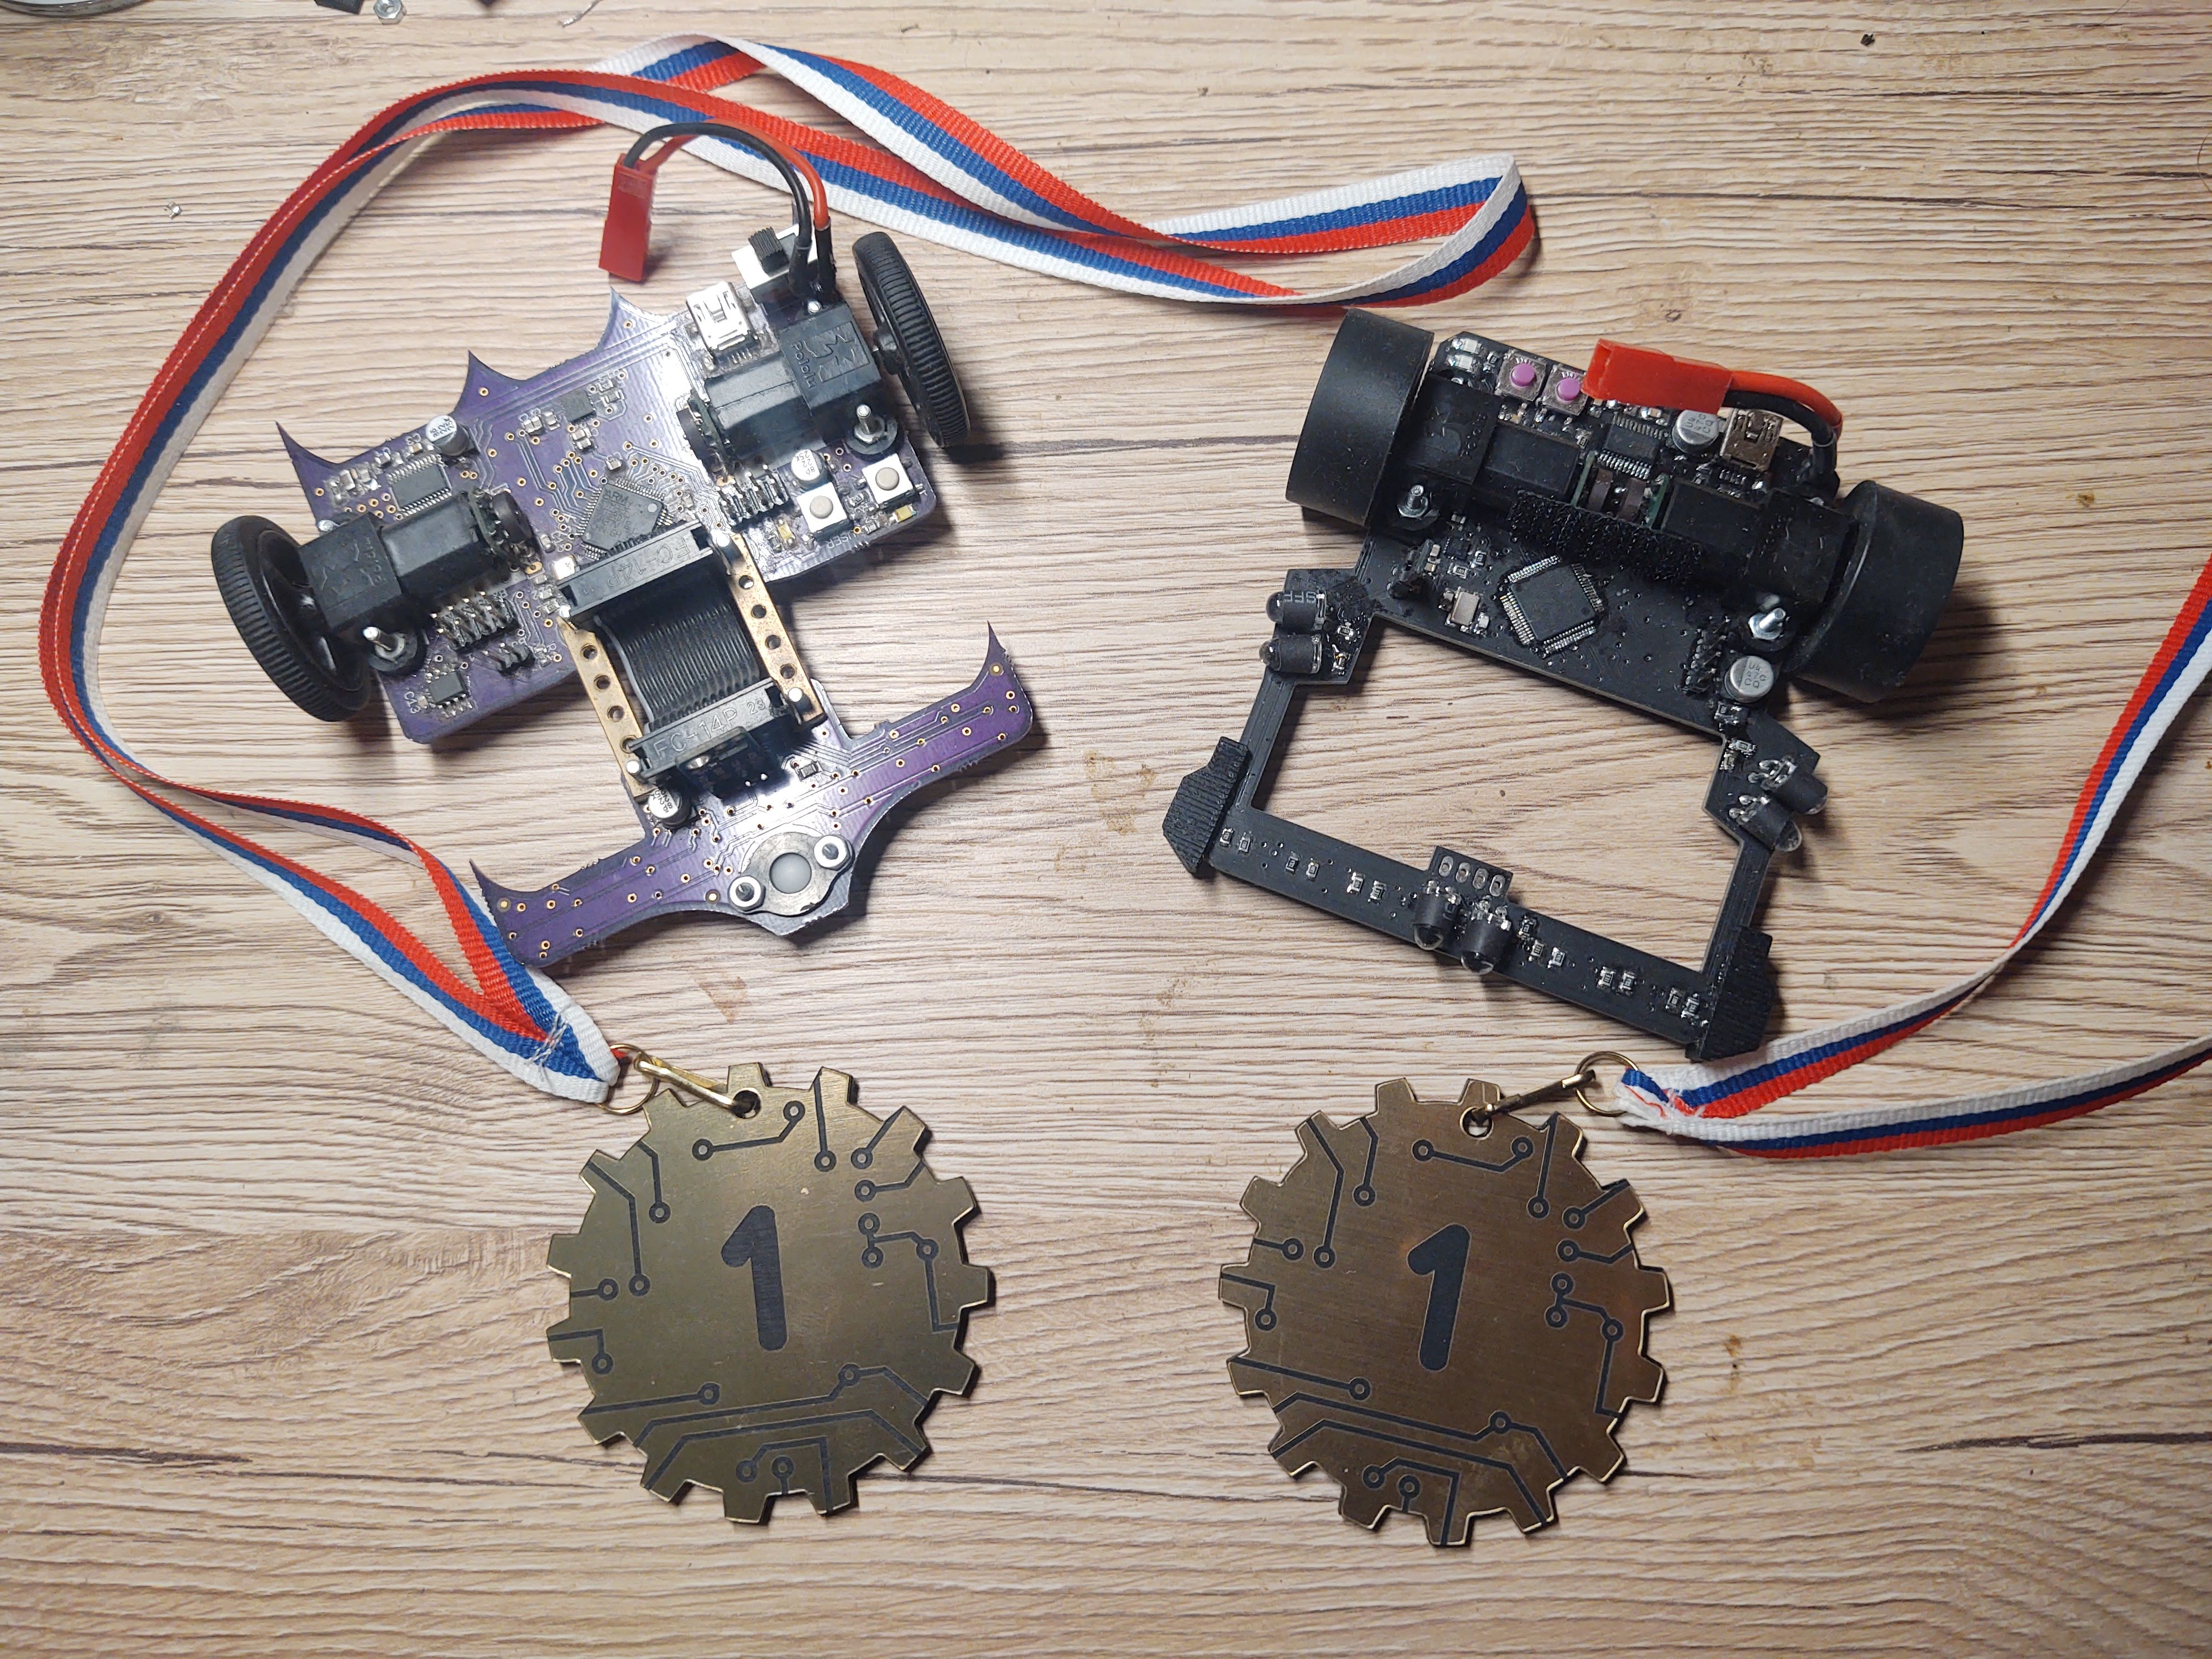
\includegraphics[scale=0.035]{../images/medals.jpg}}
    \end{column}
  \end{columns}

  video : \url{https://www.youtube.com/watch?v=xUAJ1LA6Xwc}

\end{frame}




\begin{frame}{\bf unsolved problems}

  \begin{itemize}
    \item RL sample efficiency
    \item sparse rewards
    \item generalisation
  \end{itemize}
  
  \end{frame}
  
  \begin{frame}{\bf Montezuma's revenge}
  
    \centering{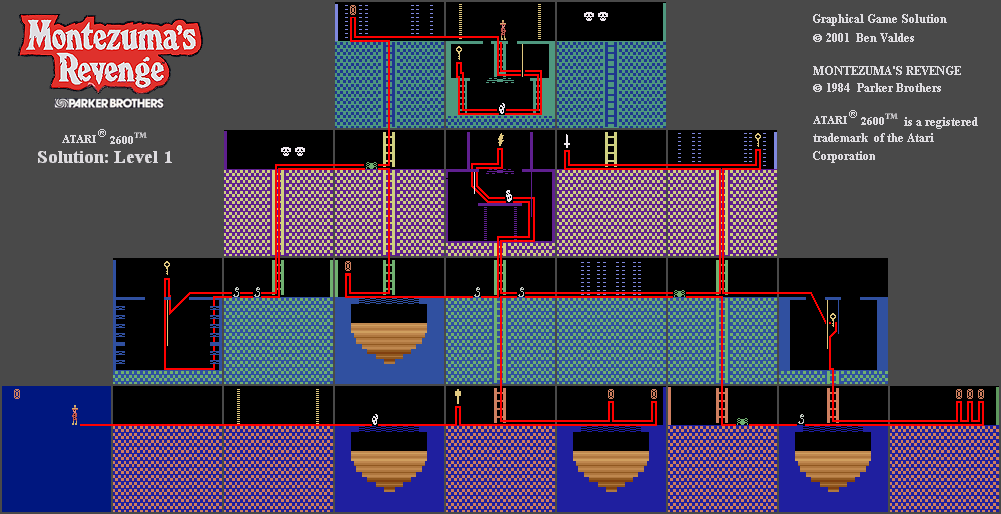
\includegraphics[scale=0.3]{../images/montezuma_map.png}}
  
    \begin{itemize}
      \item extreme sparse rewards
      \item huge state space
      \item need to return hundrets of steps back
      \item still not solved - without game state save/load
    \end{itemize}
  
  \end{frame}
  
  
  \begin{frame}{\bf state of the art score}
  
  \begin{columns}
      \column{\dimexpr\paperwidth-10pt}
  
        source : \url{https://paperswithcode.com/sota/atari-games-on-atari-2600-montezumas-revenge}
  
  
        \begin{table}[]
        \begin{tabular}{|l|l|l|}
        \hline
        \textbf{year} & \textbf{name}                                       & \textbf{score} \\ \hline
        2015          & Deep Reinforcement Learning with Double Q-learning  & 0              \\ \hline
        2017          & Curiosity-driven Exploration by Self-supervised Prediction \footnote[1]{https://arxiv.org/abs/1705.05363} & 0       \\ \hline 
        2021          & MuZero                                              & 2500           \\ \hline
        2018          & Count-Based Exploration with Neural Density Models \footnote[2]{https://arxiv.org/abs/1703.01310}  & 3705           \\ \hline
        \textbf{2019} & \textbf{Exploration by Random Network Distillation} \footnote[3]{https://arxiv.org/abs/1810.12894}& \textbf{8152}  \\ \hline
        2021          & GoExplore$^*$ \footnote[4]{https://arxiv.org/abs/2004.12919}                         & 43 000         \\ \hline
        \end{tabular}
        \end{table}
  
        {\bf * requires environment state saving/loading}
  
  \end{columns}
  
  \end{frame}
  

\begin{frame}{\bf exploration by self supervised exploitation}

  \centering{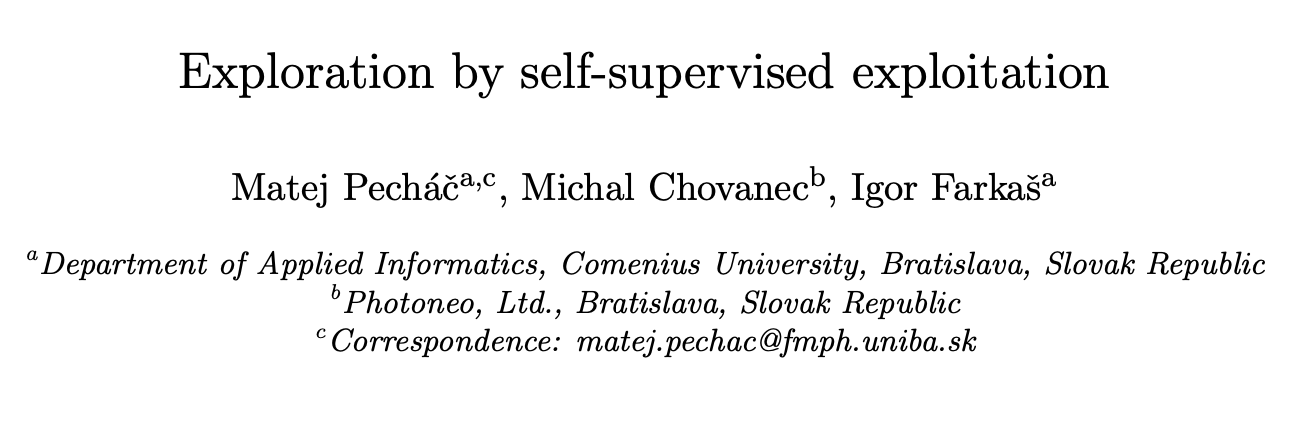
\includegraphics[scale=0.4]{../images/cnd.png}}

  \begin{itemize}
    \item self supervised model regularisation
    \item reached state of the art score (25 000 +) on Montezuma's Revenge
    \item first algorithm solving procgen hard exploration seeds
  \end{itemize} 
\end{frame}
  

\begin{frame}
  
  \frametitle{\bf recommended sources}

  \begin{itemize}
    \item book : Maxim Lapan, 2020, Deep Reinforcement Learning Hands-On second edition
    \item book : Enes Bilgin, 2020, Mastering Reinforcement Learning with Python
    \item youtuber : Yannic Kilcher, \href{https://www.youtube.com/c/YannicKilcher/videos}{link}
    \item youtuber : Two Minute Papers, \href{https://www.youtube.com/c/KárolyZsolnai/videos}{link}
    \item web : Paper With Code, \href{https://paperswithcode.com/methods/category/policy-gradient-methods}{link}
    \item web : Intellabs, \href{https://intellabs.github.io/coach/components/agents/index.html}{link}
  \end{itemize}

 
    
\end{frame}



\begin{frame}
  
  \frametitle{Q\&A}

  \begin{columns}

    \begin{column}{0.5\textwidth}
      \centering{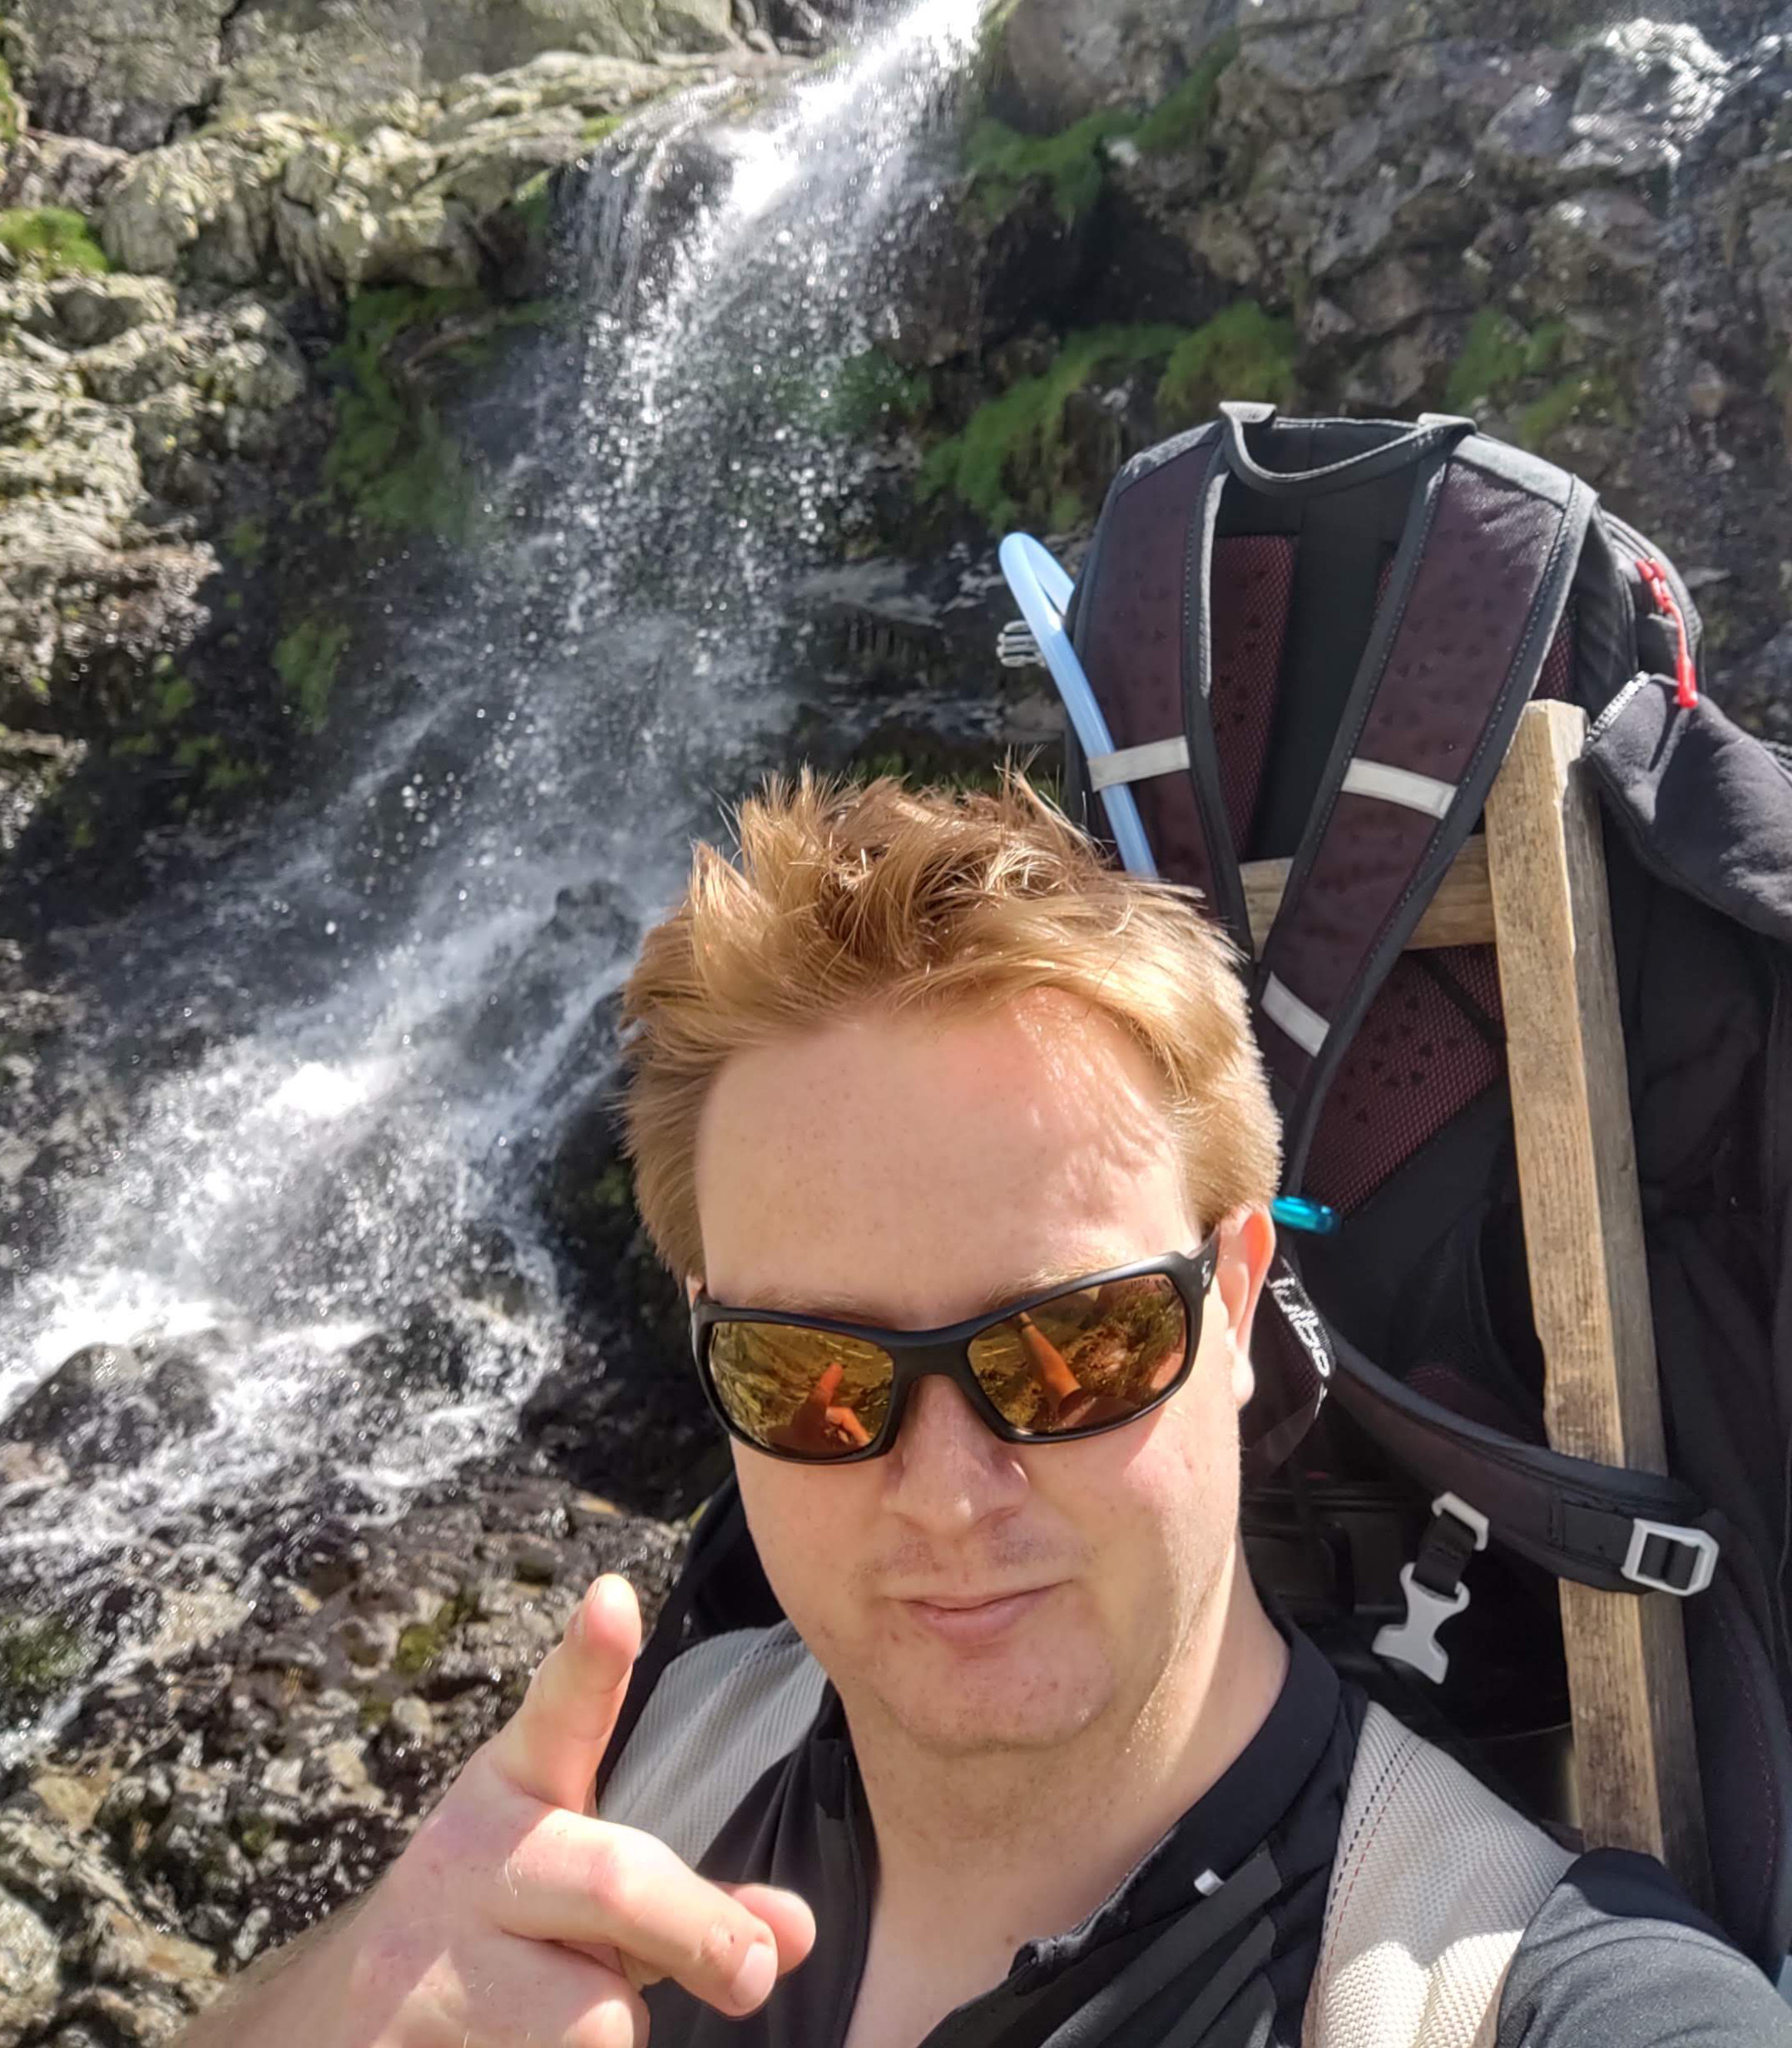
\includegraphics[scale=0.08]{../images/me.jpg}}
    \end{column}

    \begin{column}{0.5\textwidth}
      \begin{itemize}
        \item \url{https://github.com/michalnand/}
        \item \url{michal.nand@gmail.com}
      \end{itemize}
    \end{column}

  \end{columns}

    
\end{frame}

\end{document}